\providecommand{\toplevelprefix}{../..}  %
\documentclass[../../book-main.tex]{subfiles}

\begin{document}

\chapter{An Informal Introduction}
\label{ch:intro}

\begin{quote}
``{\em Just as the constant increase of entropy is the basic law of the universe, so it is the basic law of life to be ever more highly structured and to struggle against entropy.}''

$~$\hfill -- V\'{a}clav Havel
 \end{quote}
\vspace{5mm}



\section{Intelligence, Cybernetics, and Artificial Intelligence}
The world we inhabit is neither fully random nor completely unpredictable.\footnote{If the world were fully random, an intelligent being would have no need to learn or memorize anything.} Instead, it follows certain orders, patterns, and laws that render it largely predictable.\footnote{Some deterministic, some probabilistic.} The very emergence and persistence of life depend on this predictability. Only by learning and memorizing what is predictable in the environment can life survive and thrive, since sound decisions and actions hinge on reliable predictions. Because the world offers seemingly unlimited predictable phenomena, intelligent beings---animals and humans---have evolved ever more acute senses: vision, hearing, touch, taste, and smell. These senses harvest high-throughput sensory data to perceive environmental regularities. Hence, a fundamental task for all intelligent beings is to
\begin{center}
    \textit{learn and memorize predictable information from massive amounts of sensed data}.
\end{center}
Before we can understand how this is accomplished, we must address three questions:
\begin{itemize}
    \item How can predictable information be modeled and represented mathematically?
    \item How can such information be computationally learned effectively and efficiently from data?
    \item How should this information be best organized to support future prediction and inference?
\end{itemize}
This book aims to provide some answers to these questions. These answers will help us better understand intelligence, especially the computational principles and mechanisms that enable it. Evidence suggests that all forms of intelligence---from low-level intelligence seen in early primitive life to the highest form of intelligence, the practice of modern science---share a common set of principles and mechanisms. We elaborate below.

\paragraph{Emergence and evolution of intelligence.}

A necessary condition for the emergence of life on Earth about four billion years ago is that the environment is largely predictable. Life has developed mechanisms that allow it to learn what is predictable about the environment, encode this information, and use it for survival. Generally speaking, we call this ability to learn knowledge of the world \textit{intelligence}. To a large extent, the evolution of life is the mechanism of intelligence at work \cite{Bennett-2023}. In early stages of life, intelligence is mainly developed through two types of learning mechanisms: \textit{phylogenetic} and \textit{ontogenetic} \cite{Wiener-Cybernetics-1961}.

\textit{Phylogenetic intelligence} refers to learning through the evolution of species. Species inherit and survive mainly based on knowledge encoded in the DNA or genes of their parents. To a large extent, we may call DNA nature's pre-trained large models because they play a very similar role. The main characteristic of phylogenetic intelligence is that individuals have limited learning capacity. Learning is carried out through a ``trial-and-error'' mechanism based on random mutation of genes, and species evolve based on natural selection---survival of the fittest---as shown in \Cref{fig:phylogenetic}. This can be viewed as nature's implementation of what is now known as ``reinforcement learning,'' \cite{Sutton-Barto} or potentially ``neural architecture search'' \cite{NAS-1}. However, such a ``trial-and-error'' process can be extremely slow, costly, and unpredictable. From the emergence of the first life forms, about 4.4--3.8 billion years ago \citep{bell2015potentially}, life has relied on this form of evolution.\footnote{Astute readers may notice an uncanny similarity between how early life evolves and how large language models evolve today.}

\begin{figure}
    \centering
    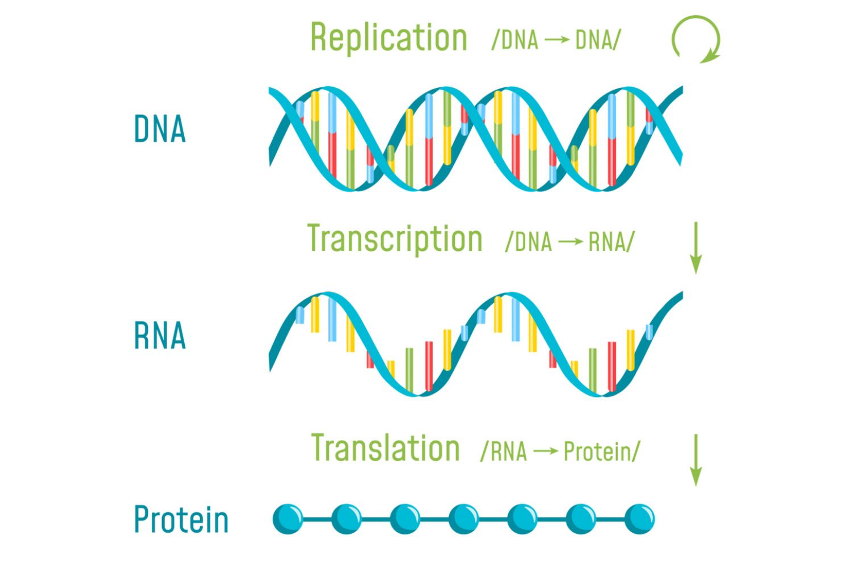
\includegraphics[width=0.5\linewidth]{\toplevelprefix/chapters/chapter1/figs/DNAs.png}
    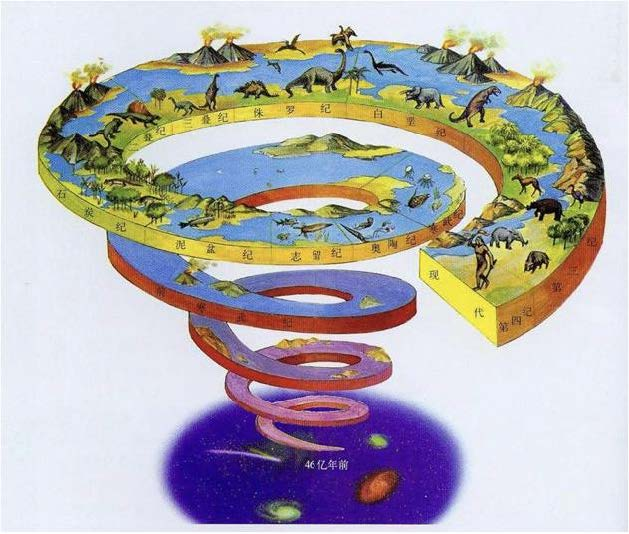
\includegraphics[width=0.40\linewidth]{\toplevelprefix/chapters/chapter1/figs/Evolution.jpg}
    \caption{Evolution of phylogenetic intelligence: Knowledge of the external world is encoded and passed on via DNA (left), and decoded from DNA to RNA and to proteins. In the early stage of life evolution (right), intelligence develops knowledge at the species level via (random) gene mutation and natural selection---``may the fittest survive''---which can be viewed as a primitive form of reinforcement learning.}
    \label{fig:phylogenetic}
\end{figure}

\begin{figure}
    \centering
    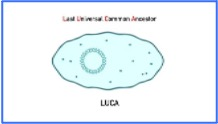
\includegraphics[height=0.19\linewidth]{\toplevelprefix/chapters/chapter1/figs/Luca.jpeg}
    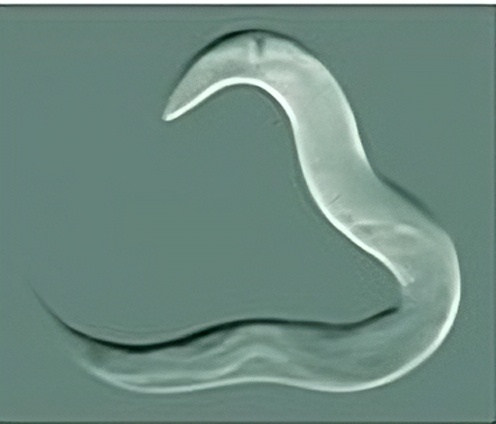
\includegraphics[height=0.19\linewidth]{\toplevelprefix/chapters/chapter1/figs/Worm.jpeg}
    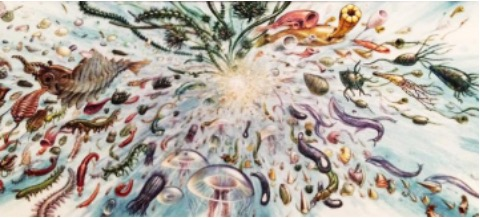
\includegraphics[height=0.19\linewidth]{\toplevelprefix/chapters/chapter1/figs/Cambrian.jpg}
    \caption{Evolution of life, from the ancestor of all life today (LUCA---last universal common ancestor), a single-cell-like organism that lived 3.5--4.3 billion years ago \cite{moody2024nature}, to the emergence of the first nervous system in worm-like species (middle), about 550 million years ago \cite{wang2025preservation}, to the explosion of life forms in the Cambrian period (right), about 530 million years ago.}
    \label{fig:evolution}
\end{figure}

\textit{Ontogenetic intelligence} refers to the learning mechanisms that allow an individual to learn through its own senses, memories, and predictions within its specific environment, and to improve and adapt its behaviors. Ontogenetic learning became possible after the emergence of the nervous system about 550--600 million years ago (in worm-like organisms) \cite{wang2025preservation}, shown in \Cref{fig:evolution} middle. With a sensory and nervous system, an individual can continuously form and improve its own knowledge about the world (memory), in addition to what is inherited from DNA or genes. This capability significantly enhanced individual survival and contributed to the Cambrian explosion of life forms about 530 million years ago \cite{Parker-2004}. Compared to phylogenetic learning, ontogenetic learning is more efficient and predictable, and can be realized within an individual's resource limits.

Both types of learning rely on feedback from the external environment---penalties (death) or rewards (food)---applied to a species' or an individual's actions.\footnote{Gene mutation of the species or actions made by the individual.} This insight inspired Norbert Wiener to conclude in his Cybernetics program \cite{Wiener-Cybernetics-1948} that all intelligent beings, whether species or individuals, rely on closed-loop feedback mechanisms to learn and improve their knowledge about the world. Furthermore, from plants to fish, birds, and mammals, more advanced species increasingly rely on ontogenetic learning: they remain with and learn from their parents for longer periods after birth, because individuals of the same species must survive in very diverse environments.

\paragraph{Evolution of human intelligence.}
Since the emergence of \textit{Homo sapiens} about 2.5 million years ago \cite{Harari-2015}, a new, higher form of intelligence has emerged that evolves more efficiently and economically. Human societies developed languages---first spoken, later written---as shown in \Cref{fig:human-intelligence}. Language enables individuals to communicate and share useful information, allowing a human community to behave as a single intelligent organism that learns faster and retains more knowledge than any individual. Written texts thus play a role analogous to DNA and genes, enabling societies to accumulate and transmit knowledge across generations. We may refer to this type of intelligence as \textit{societal intelligence}, distinguishing it from the phylogenetic intelligence of species and the ontogenetic intelligence of individuals. This knowledge accumulation underpins (ancient) civilizations.

\begin{figure}
    \centering
    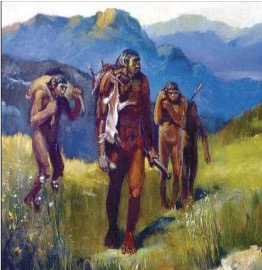
\includegraphics[height=0.25\linewidth]{\toplevelprefix/chapters/chapter1/figs/Spoken-language.jpg}
   \hspace{5mm} 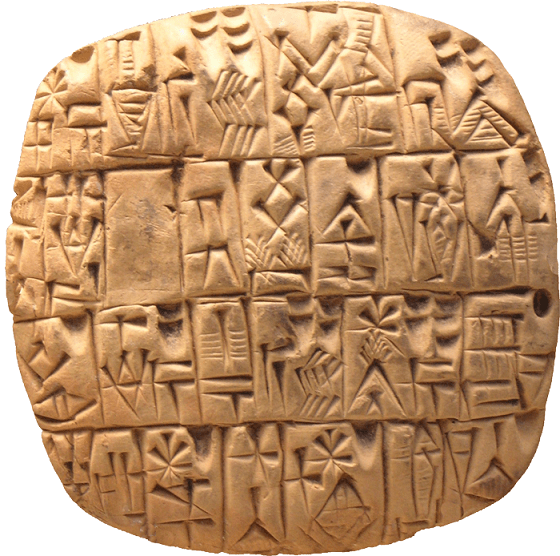
\includegraphics[height=0.25\linewidth]{\toplevelprefix/chapters/chapter1/figs/Cuneiform.png}
   \hspace{5mm} 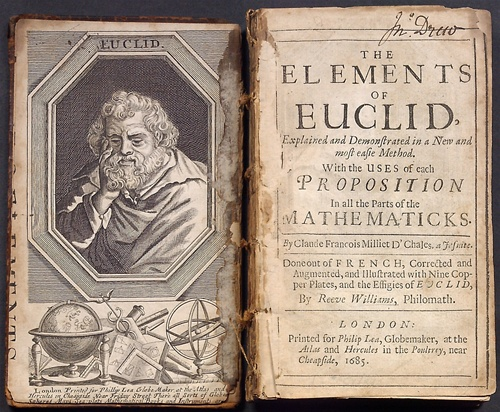
\includegraphics[height=0.25\linewidth]{\toplevelprefix/chapters/chapter1/figs/adopt-euclid1685-2.jpg}
    \caption{The development of verbal communication and spoken languages (70,000--30,000 years ago), written languages (about 3000 BC) \cite{schmandt2014evolution}, and abstract mathematics (around 500--300 BC) \cite{heath1956thirteen} mark three key milestones in the evolution of human intelligence.}
    \label{fig:human-intelligence}
\end{figure}

About two to three thousand years ago, human intelligence took another major leap, enabling philosophers and mathematicians to develop knowledge that goes far beyond organizing empirical observations. The development of abstract concepts and symbols, such as numbers, time, space, logic, and geometry, gave rise to an entirely new and rigorous language of \textit{mathematics}. In addition, the development of the ability to generate hypotheses and verify their correctness through logical deduction or experimentation laid the foundation for modern \textit{science}. For the first time, humans could proactively and systematically discover and develop new knowledge. We will call this advanced form of intelligence ``scientific intelligence'' due to its necessity for deductive and scientific discovery.

Hence, from what we can learn from nature, whenever we use the word ``intelligence,'' we must be specific about which level or form we mean:
\begin{equation}
    \text{\textbf{phylogenetic}} \;
   \Longrightarrow \; \text{\textbf{ontogenetic}} \; \Longrightarrow \; 
   \text{\textbf{societal}}
   \; \Longrightarrow \; 
   \text{\textbf{scientific intelligence}}.
\end{equation}
Clear characterization and distinction are necessary because we want to study intelligence as a scientific and mathematical subject. Although all forms may share the common objective of learning useful knowledge about the world, the specific computational mechanisms and physical implementations behind each level could differ. We believe the reader will better understand and appreciate these differences after studying this book. Therefore, we leave further discussion of general intelligence to the last \Cref{ch:future}.

\paragraph{Origin of machine intelligence---cybernetics.}
In the 1940s, spurred by the war effort, scientists inspired by natural intelligence sought to emulate animal intelligence with machines, giving rise to the ``Cybernetics'' movement championed by Norbert Wiener \cite{Kline-2011}. Wiener studied zoology at Harvard as an undergraduate before becoming a mathematician and control theorist. He devoted his life to understanding and building autonomous systems that could reproduce animal-like intelligence. Today, the Cybernetics program is often narrowly interpreted as being mainly about feedback control systems, the area in which Wiener made his most significant technical contributions. Yet the program was far broader and deeper: it aimed to understand intelligence as a whole---at least at the animal level---and influenced the work of an entire generation of renowned scientists, including Warren McCulloch, Walter Pitts, Claude Shannon, John von Neumann, and Alan Turing.

\begin{figure}
    \centering
    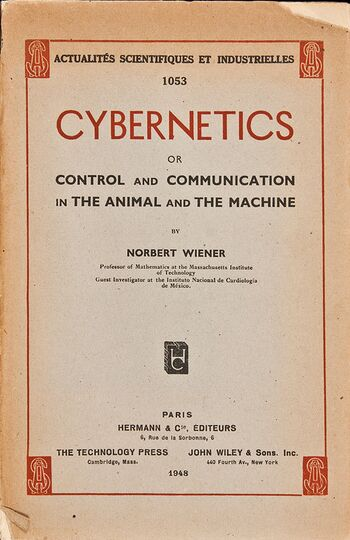
\includegraphics[height=0.4\linewidth]{\toplevelprefix/chapters/chapter1/figs/Cybernetics1.jpg}
    \hspace{10mm} 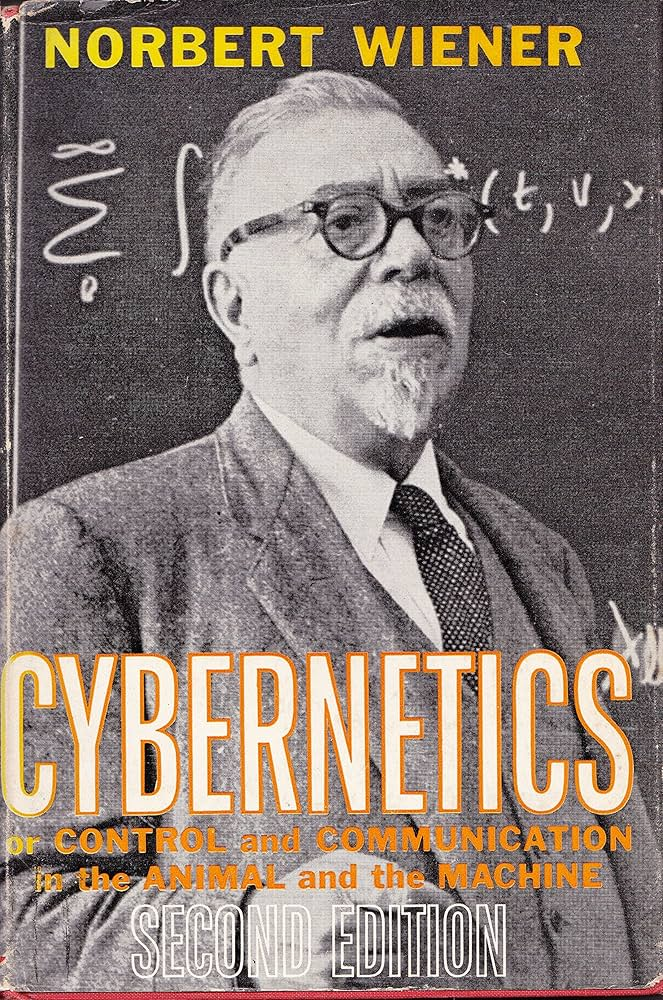
\includegraphics[height=0.4\linewidth]{\toplevelprefix/chapters/chapter1/figs/Cybernetics2.jpg}
    \caption{Norbert Wiener's book ``Cybernetics'' (1948) \cite{Wiener-Cybernetics-1948} (left) and its second edition (1961) \cite{Wiener-Cybernetics-1961} (right).}
    \label{fig:cybernetcis}
\end{figure}

Wiener was arguably the first to study intelligence \textit{as a system}, rather than focusing on isolated components or aspects of intelligence. His comprehensive views appeared in the celebrated 1948 book \textit{Cybernetics: or Control and Communication in the Animal and the Machine} \cite{Wiener-Cybernetics-1948}. In that book and its second edition published in 1961 \cite{Wiener-Cybernetics-1961} (see \Cref{fig:cybernetcis}), he attempted to identify several necessary characteristics and mechanisms of intelligent systems, including (but not limited to):
\begin{itemize}
    \item How to \textit{measure and store} information (in the brain) and how to communicate with others.\footnote{Wiener was the first to point out that ``information'' is neither matter nor energy, but an independent quantity worthy of study.} This insight led Claude Shannon to formulate \textit{information theory} in 1948 \cite{Shannon-1948}.
    \item How to \textit{correct errors} in prediction and estimation based on existing information. Wiener himself helped formalize the theory of (closed-loop) feedback control in the 1940s.
    \item How to learn to \textit{make better decisions} when interacting with a non-cooperative or even adversarial environment. John von Neumann formalized this as \textit{game theory} in 1944 \cite{von-Neumann-1944}.
\end{itemize}
In 1943, inspired by Wiener's Cybernetics program, cognitive scientist Warren McCulloch and logician Walter Pitts jointly formalized the first computational model of a neuron \cite{McCulloch-Pitts}, called an \textit{artificial neuron} and illustrated later in \Cref{fig:neuron}. Building on this model, Frank Rosenblatt constructed the Mark I Perceptron in the 1950s---a physical machine containing hundreds of such artificial neurons \cite{Rosenblatt:1957}. The Perceptron was the first physically realized artificial neural network; see \Cref{fig:perceptron}. Notably, John von Neumann's universal computer architecture, proposed in 1945, was also designed to facilitate the goal of building \textit{computing machines} that could physically realize the mechanisms suggested by the Cybernetics program \cite{von-Neumann-1958}.

Astute readers will notice that the 1940s were truly magical: many fundamental ideas were invented and influential theories formalized, including the mathematical model of neurons, artificial neural networks, information theory, control theory, game theory, and computing machines. \Cref{fig:god-fathers} portrays some of the pioneers. Each of these contributions has grown to become the foundation of a scientific or engineering field and continues to have tremendous impact on our lives. All were inspired by the goal of developing machines that emulate intelligence in nature. Historical records show that Wiener's Cybernetics movement influenced nearly all of these pioneers and works. To a large extent, Wiener's program can be viewed as the true predecessor of today's ``embodied intelligence'' program; in fact, Wiener himself articulated a vision for such a program with remarkable clarity and concreteness \cite{Wiener-Cybernetics-1961}.
\begin{figure}
    \centering
    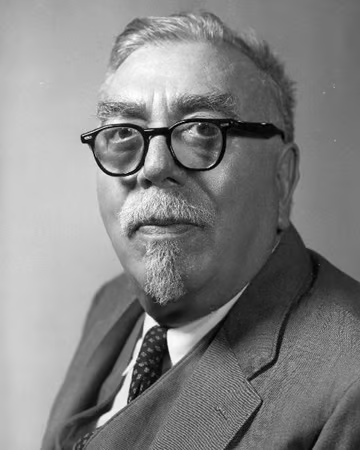
\includegraphics[height=0.3\linewidth]{\toplevelprefix/chapters/chapter1/figs/Wiener.png}
    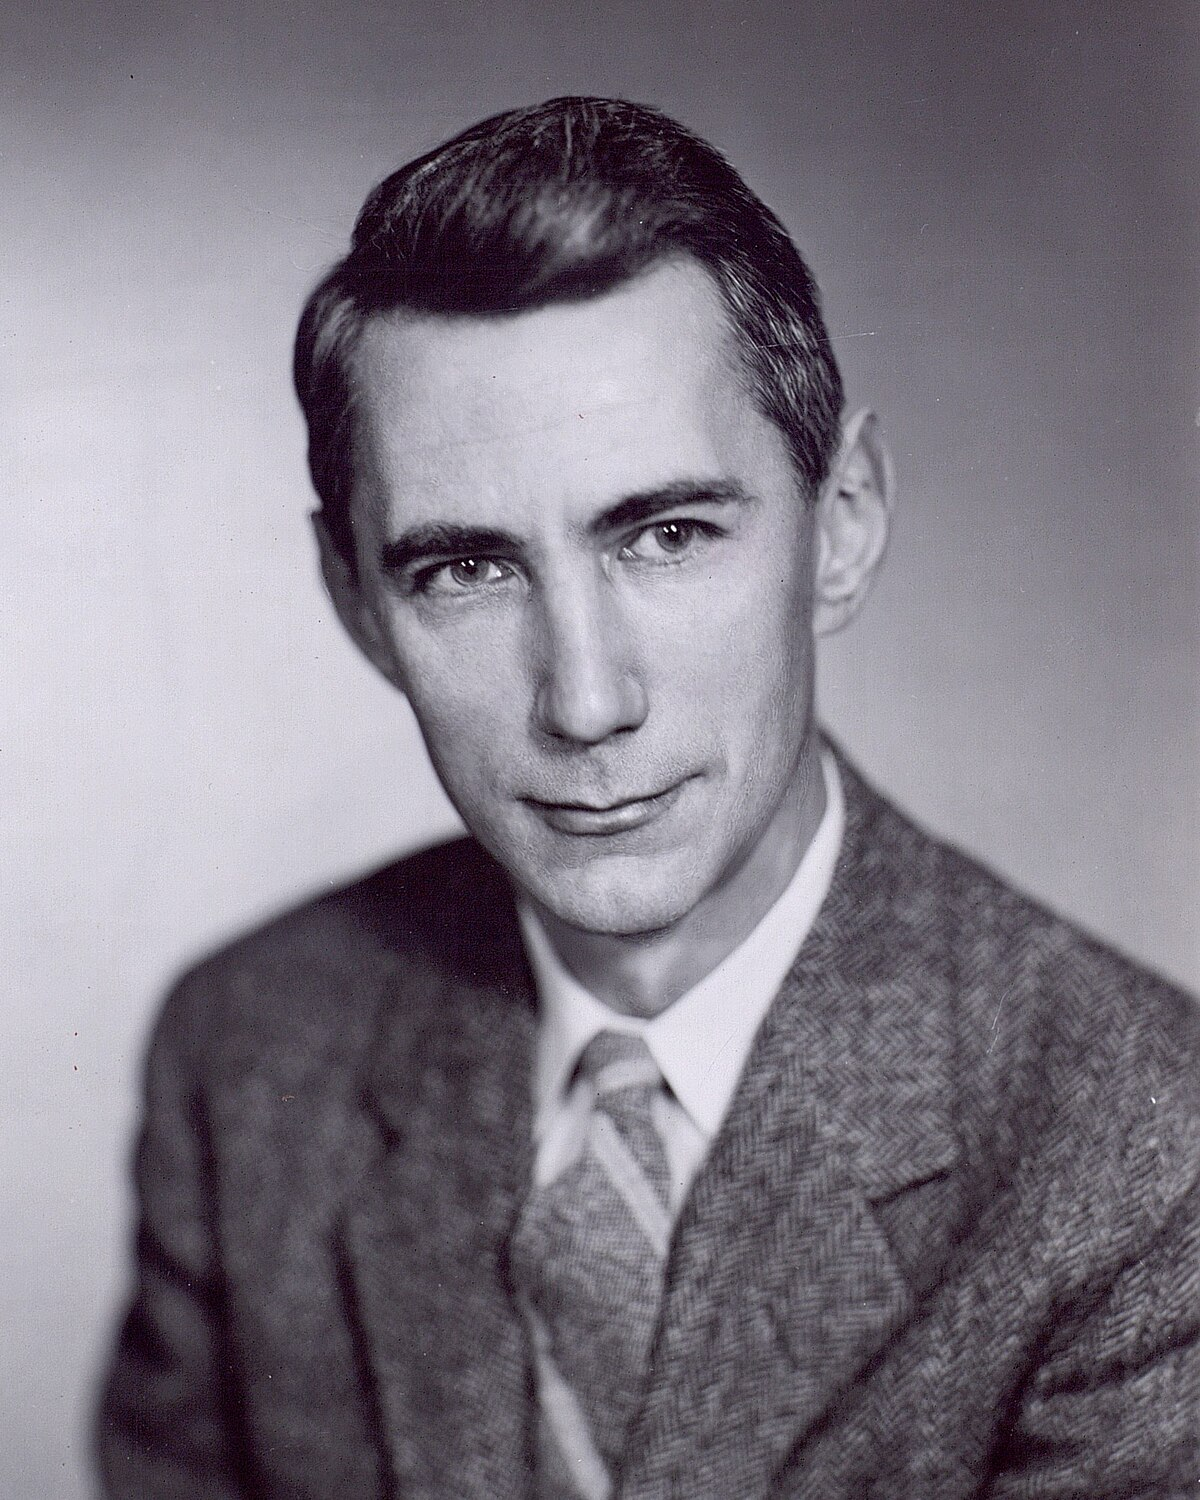
\includegraphics[height=0.3\linewidth]{\toplevelprefix/chapters/chapter1/figs/Shannon.jpg}
    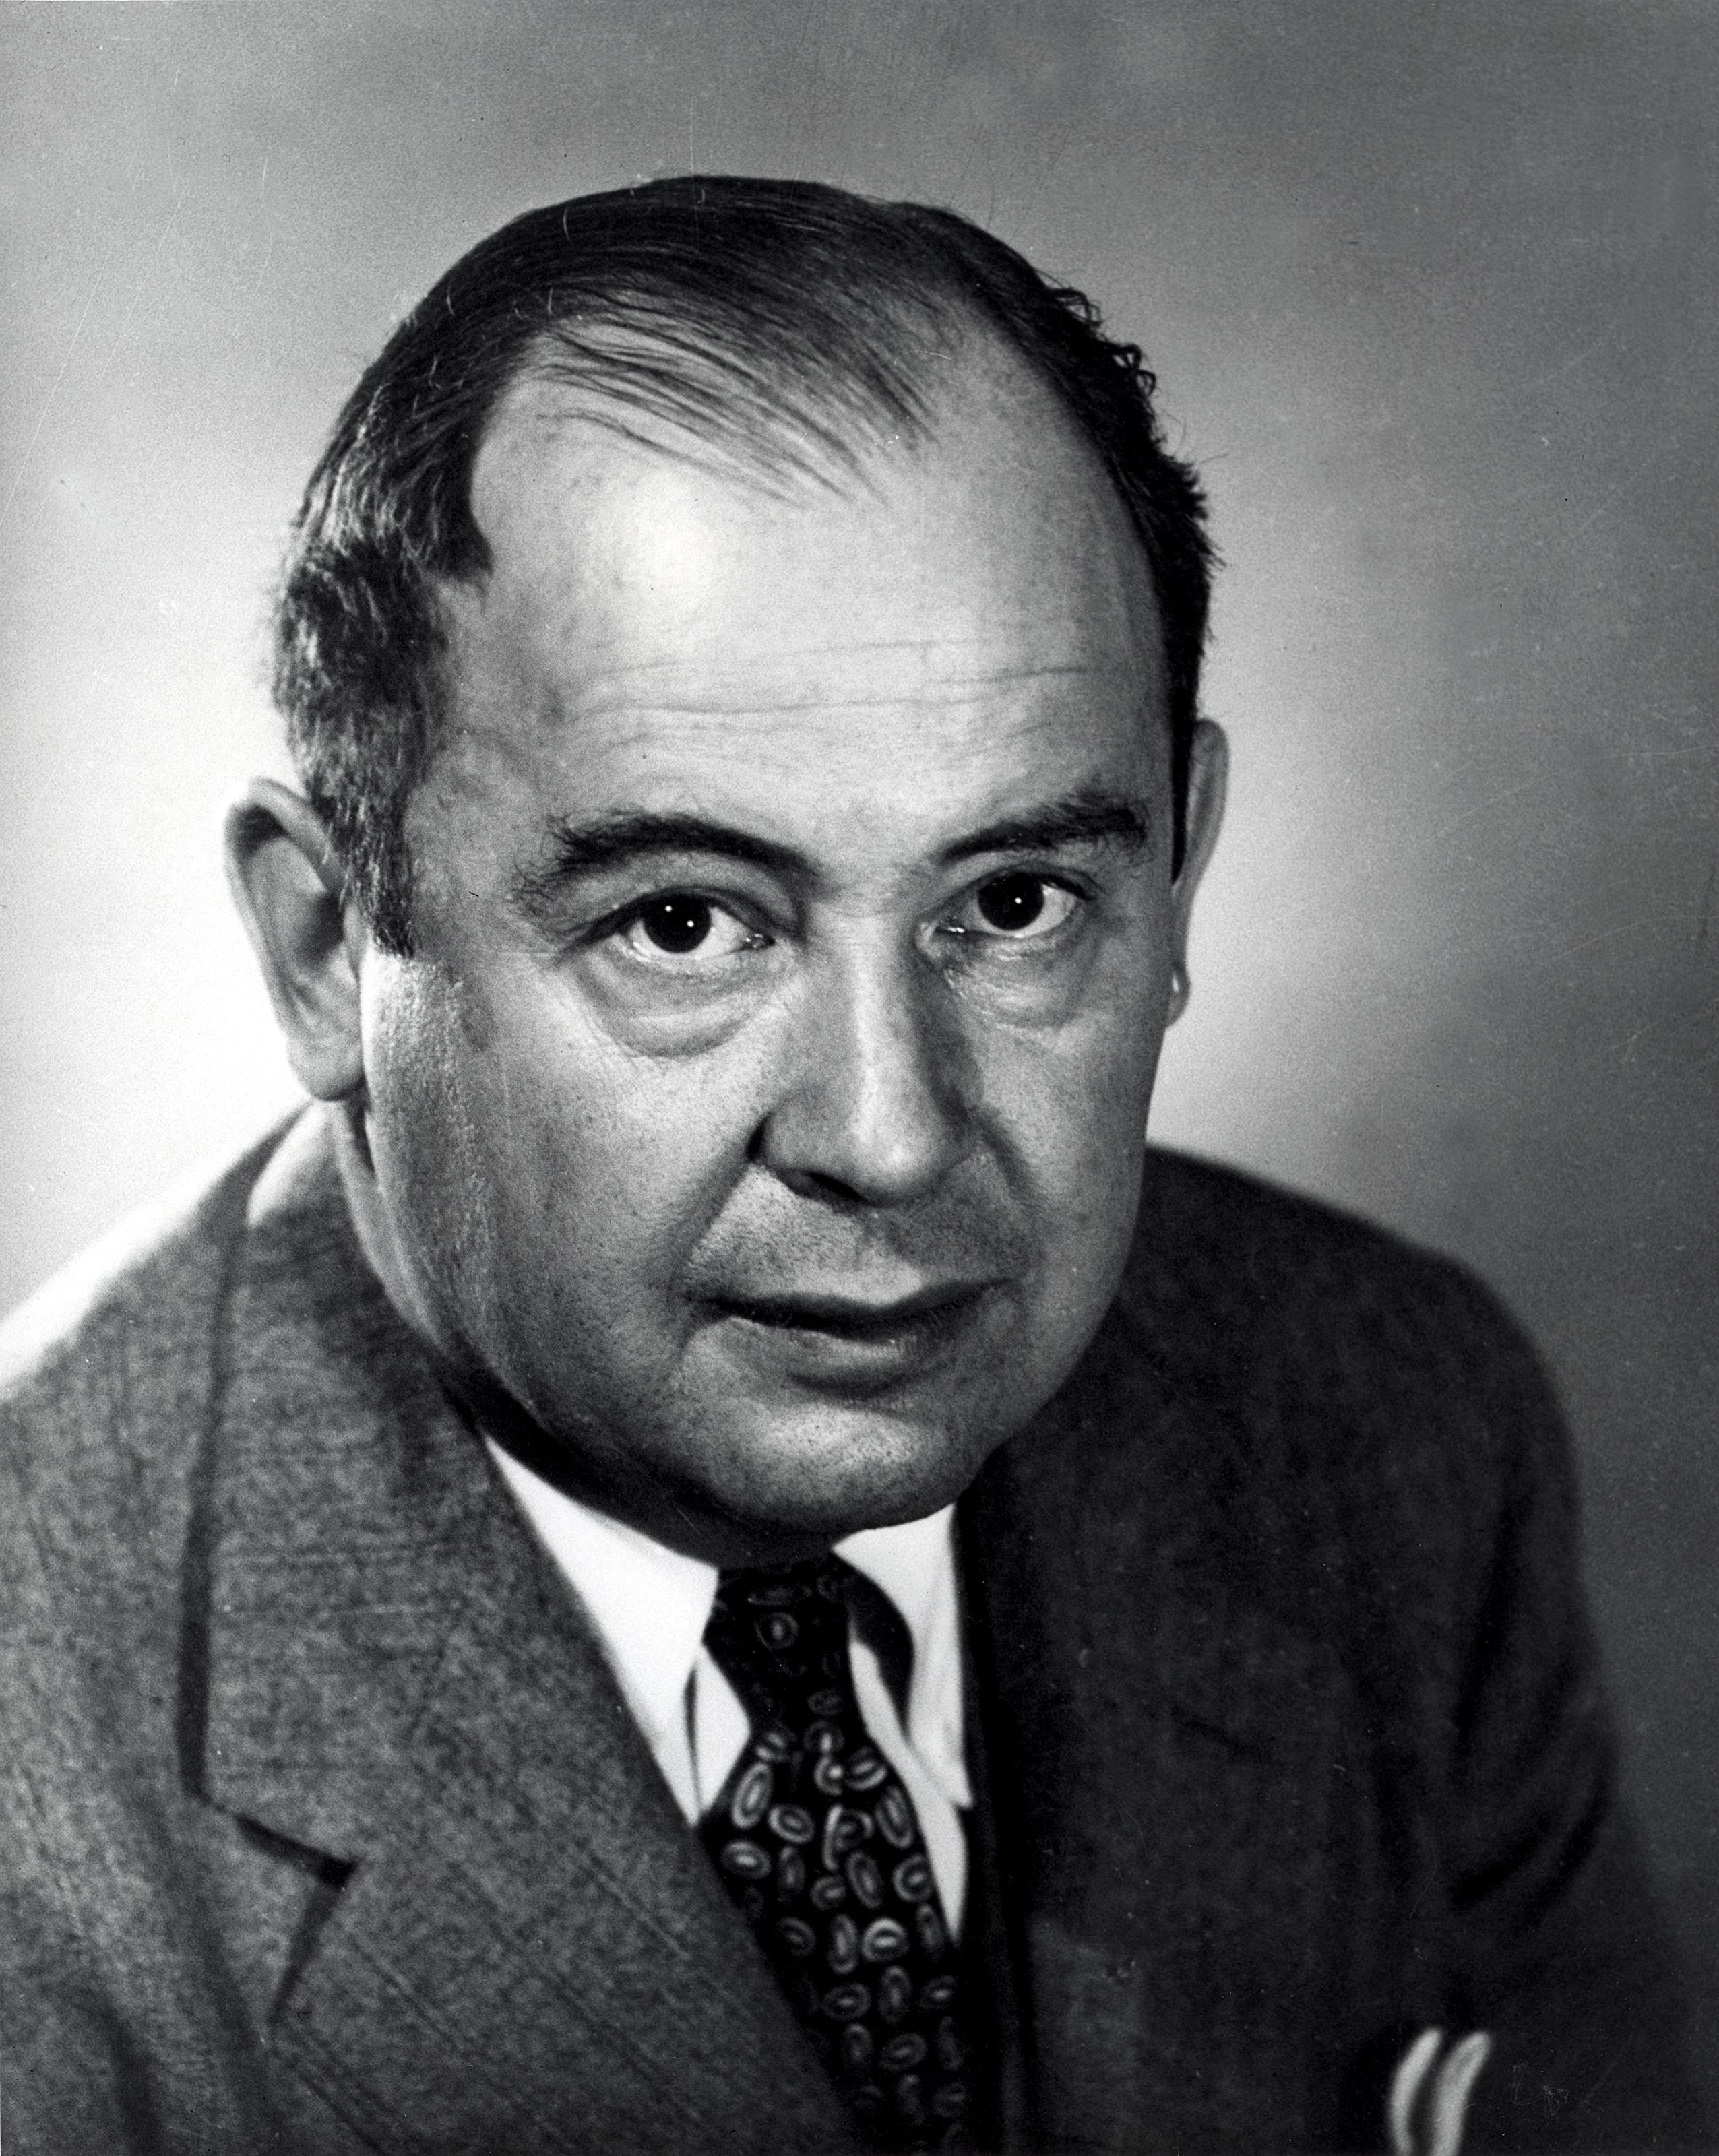
\includegraphics[height=0.3\linewidth]{\toplevelprefix/chapters/chapter1/figs/neumann.jpg}
    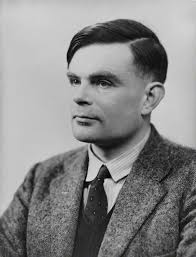
\includegraphics[height=0.3\linewidth]{\toplevelprefix/chapters/chapter1/figs/Turing.jpeg}
    \caption{Pioneers of theoretical and computational foundations for intelligence: Norbert Wiener (cybernetics and control theory), Claude Shannon (information theory), John von Neumann (game theory), and Alan Turing (computing theory).}
    \label{fig:god-fathers}
\end{figure}

Although Wiener identified many key characteristics and mechanisms of (embodied) intelligence, he offered no clear recipe for integrating them into a complete autonomous intelligent system. From today's perspective, some of his views were incomplete or inaccurate. In particular, in the last chapter of the second edition of \textit{Cybernetics} \cite{Wiener-Cybernetics-1961}, he stressed the need to \textit{deal with nonlinearity} if machines are to emulate typical learning mechanisms in nature, yet he provided no concrete, effective solution for this difficult issue. In fairness, even the theory of linear systems was in its infancy at the time, and nonlinear systems seemed far less approachable.

Nevertheless, we cannot help but marvel at Wiener's prescience. about the importance of nonlinearity. As this book will show, the answer came only recently: nonlinearity can be handled effectively through progressive linearization and transformation realized by deep networks and representations (see \Cref{ch:representation}). Moreover, we will demonstrate in this book how all the mechanisms listed above can be naturally integrated into a complete system which exhibits certain characteristics of an autonomous intelligent system (see \Cref{ch:auto-encoding}).

\paragraph{Origin of artificial intelligence.}
The subtitle of Wiener's \textit{Cybernetics}---\textit{Control and Communication in the Animal and the Machine}---reveals that 1940s research aimed primarily at emulating animal-level intelligence. As noted earlier, the agendas of that era were dominated by Wiener's Cybernetics movement.

Alan Turing was among the first to recognize this limitation. In his celebrated 1950 paper ``\textit{Computing Machinery and Intelligence}'' \cite{Turing-1950}, Turing formally posed the question of whether machines could imitate human-level intelligence, to the point of machine intelligence being indistinguishable from human intelligence---now known as \textit{the Turing test}.

Around 1955, a group of ambitious young scientists sought to break away from the then-dominant Cybernetics program and establish their own legacy. They accepted Turing's challenge of imitating human intelligence and proposed a workshop at Dartmouth College to be held in the summer of 1956. Their proposal stated \cite{McCarthy-1955}:
\begin{quote}
    ``\textit{The study is to proceed on the basis of the conjecture that every aspect of learning or any other feature of intelligence can in principle be so precisely described that a machine can be made to simulate it. An attempt will be made to find how to make machines use language, form abstractions and concepts, solve kinds of problems now reserved for humans, and improve themselves}.''
\end{quote}
They aimed to formalize and study the higher-level intelligence that distinguishes humans from animals. Their agenda included abstraction, symbolic methods, natural language, and deductive reasoning (causal inference, logical deduction, etc.), i.e., scientific intelligence. The organizer of the workshop, John McCarthy---then a young assistant professor of mathematics at Dartmouth College---coined the now-famous term ``Artificial Intelligence'' (AI) to describe machines that exhibit scientific intelligence in order to formally describe the problems and goals of the workshop.

\paragraph{Renaissance of ``artificial intelligence'' or ``cybernetics''?}
Over the past decade, machine intelligence has undergone explosive development, driven largely by deep artificial neural networks, sparked by the 2012 work of Geoffrey Hinton and his students \cite{krizhevsky2012imagenet}. This period is hailed as the ``Renaissance of AI.'' Yet, in terms of the tasks actually tackled (recognition, generation, prediction) and the techniques developed (reinforcement learning, imitation learning, encoding, decoding, denoising, and compression), we are largely emulating mechanisms common to the intelligence of early life and animals. Even in this regard, as we will clarify in this book, current ``AI'' models and systems have not fully or correctly implemented all necessary mechanisms for intelligence at the animal level which were known to the 1940s Cybernetics movement.

Strictly speaking, the recent advances of machine intelligence in the past decade do not align well with the 1956 Dartmouth AI program. Instead, what has been achieved is closer to the objectives of Wiener's classic 1940s Cybernetics program. It is probably more appropriate to call the current era the ``Renaissance of Cybernetics.''\footnote{The recent rise of so-called ``Embodied AI'' for autonomous robots aligns even more closely with the goals of the Cybernetics program.} Only after we fully understand, from scientific and mathematical perspectives, what we have truly accomplished can we determine what remains and which directions lead to the true nature of intelligence. That is one of the main purposes of this book.


\section{What to Learn?}
\label{sec:what-to-learn}

\subsection{Predictability}
\label{sec:predictability}
Data that carry useful information manifest in many forms. In their most natural form, they can be modeled as sequences that are predictable and computable. The notion of a predictable and computable sequence was central to the theory of computing and largely led to the invention of computers \cite{Turing-1936}. The role of predictable sequences in (inductive) inference was studied by Ray Solomonoff, Andrey Kolmogorov, and others in the 1960s \cite{Kolmogorov1998OnTO} as a generalization of Claude Shannon's classic information theory \cite{Shannon-1948}. To understand the concept of predictable sequences, we begin with some concrete examples.

\paragraph{Scalar case.} The simplest predictable discrete sequence is arguably the sequence of natural numbers:
\begin{equation}
   S = 1, 2, 3, 4, 5, 6, \ldots, n, n+1, \ldots
\end{equation}
in which the next number \(x_{n+1}\) is defined as the previous number \(x_{n}\) plus 1:
\begin{equation}
    x_{n+1} = x_{n} + 1.    
\end{equation}
One may generalize the notion of predictability to any sequence \(\{x_{n}\}_{n=1}^{\infty}\) with \(x_{n} \in \R\) if the next number \(x_{n+1}\) can always be computed from its predecessor \(x_{n}\):
\begin{equation}
    x_{n+1} = f(x_{n}), \quad x_{n} \in \R, \; n = 1, 2, 3, \ldots
\end{equation}
where \(f(\cdot)\) is a \textit{computable} (scalar) function.\footnote{Here we emphasize that the function \(f(\cdot)\) itself is computable, meaning it can be implemented as a program on a computer.} Alan Turing's seminal work in 1936 \cite{Turing-1936} gives a rigorous definition of computability. In practice, we often further assume that \(f\) is efficiently computable and has nice properties such as continuity and differentiability. The necessity of these properties will become clear later once we understand more refined notions of computability and their roles in machine learning and intelligence.

\paragraph{Multivariable case.}
The next value may also depend on two predecessors. For example, the famous \textit{Fibonacci sequence}
\begin{equation}
    S = 1, 1, 2, 3, 5, 8, 13, 21, 34, 55, \ldots
\end{equation}
satisfies
\begin{equation}
    x_{n+2} = x_{n+1} + x_{n}, \quad x_{n} \in \R, \; n = 1, 2, 3, \ldots
\end{equation}
More generally, we may write
\begin{equation}
    x_{n+2} = f(x_{n+1}, x_{n}), \quad x_{n} \in \R, \; n = 1, 2, 3, \ldots
\end{equation}
for any computable function \(f\) that takes two inputs. Extending further, the next value may depend on the preceding \(d\) values:
\begin{equation}
    x_{n+d} = f(x_{n+d-1}, \ldots, x_{n}), \quad x_{n} \in \R, \; n = 1, 2, 3, \ldots
    \label{eqn:recursive-d}
\end{equation}
The integer \(d\) is called the \textit{degree} of the recursion. The above expression \eqref{eqn:recursive-d} is called an \textit{autoregression}, and the resulting sequence is \textit{autoregressive}. When \(f\) is linear, we say it is a \textit{linear autoregression}.

\paragraph{Vector case.}
To simplify notation, we define a vector \(\vx \in \R^{d}\) that collects \(d\) consecutive values in the sequence:
\begin{equation}
    \vx_{n} \doteq [x_{n+d-1}, \ldots, x_{n}]^{\top}, \quad \vx_{n} \in \R^{d}, \; n = 1, 2, 3, \ldots
\end{equation}
With this notation, the recursive relation \eqref{eqn:recursive-d} becomes
\begin{equation}
    \vx_{n+1} = g(\vx_{n}) \in \R^{d}, \quad n = 1, 2, 3, \ldots
    \label{eqn:recursive-v}
\end{equation}
where \(g(\cdot)\) is uniquely determined by the function \(f\) in \eqref{eqn:recursive-d} and maps a \(d\)-dimensional vector to a \(d\)-dimensional vector. In different contexts, such a vector is sometimes called a ``state'' or a ``token.'' Note that \eqref{eqn:recursive-d} defines a mapping \(\R^{d} \to \R\), whereas here we have \(g \colon \R^{d} \to \R^{d}\).

\paragraph{Controlled prediction.}
We may also define a predictable sequence that depends on another predictable sequence as input:
\begin{equation}
    \vx_{n+1} = f(\vx_{n}, \vu_{n}) \in \R^{d}, \quad n = 1, 2, 3, \ldots,
    \label{eqn:recursive-control}
\end{equation}
where \(\{\vu_{n}\}\) with \(\vu_{n} \in \R^{k}\) is a (computable) predictable sequence. In other words, the next vector \(\vx_{n+1} \in \R^{d}\) depends on both \(\vx_{n} \in \R^{d}\) and \(\vu_{n} \in \R^{k}\). In control theory, the sequence \(\{\vu_{n}\}\) is often referred to as the ``control input'' and \(\vx_{n}\) as the ``state'' or ``output'' of the system \eqref{eqn:recursive-control}. A classic example is a linear dynamical system:
\begin{equation}
    \vx_{n+1} = \vA\vx_{n} + \vB\vu_{n}, \quad \vA \in \R^{d \times d}, \vB \in \R^{d \times k},
    \label{eqn:lineary-system} 
\end{equation}
which is widely studied in control theory \cite{Cal:Des}. 

Often the control input is given by a computable function of the state \(\vx_{n}\) itself: 
\begin{equation}
    \vu_{n} = h(\vx_{n}), \quad n = 1, 2, 3, \ldots 
    \label{eqn:control-function}
\end{equation}
As a result, the sequence \(\{\vx_{n}\}\) is given by composing the two computable functions \(f\) and \(h\):
\begin{equation}
    \vx_{n+1} = f(\vx_{n}, h(\vx_{n})), \quad n = 1, 2, 3, \ldots
    \label{eqn:recursive-closed-loop}
\end{equation}
In this way, the sequence \(\{\vx_{n}\}\) again becomes an autoregressive predictable sequence. When the input \(\vu_{n}\) depends on the output \(\vx_{n}\), we say the resulting sequence is produced by a ``closed-loop'' system \eqref{eqn:recursive-closed-loop}. As the closed-loop system no longer depends on any external input, we say such a system has become \textit{autonomous}. It can be viewed as a special case of autoregression. For instance, if we choose \(\vu_{n} = \vF\vx_{n}\) in the above linear system \eqref{eqn:lineary-system}, the closed-loop system becomes
\begin{equation}
    \vx_{n+1} = \vA\vx_{n} + \vB\vu_{n} = \vA\vx_{n} + \vB\vF\vx_{n} = (\vA + \vB\vF)\vx_{n},
    \label{eqn:lineary-system-closed}
\end{equation}
which is a linear autoregression.


\paragraph{Continuous processes.}
Predictable sequences have natural continuous counterparts, which we call predictable processes. The simplest such process is time itself, \(x(t) = t\).

More generally, a process \(\vx(t)\) is \textit{predictable} if, at every time \(t\), its value at \(t + \delta t\) is determined by its value at \(t\), where \(\delta t\) is an infinitesimal increment. Typically, \(\vx(t)\) is continuous and smooth, so the change \(\delta \vx(t) = \vx(t + \delta t) - \vx(t)\) is infinitesimally small. Such processes are typically described by (multivariate) differential equations
\begin{equation}
    \dot{\vx}(t) = f(\vx(t)), \quad \vx \in \R^{d}.
    \label{eqn:process}
\end{equation}
In systems theory \cite{Cal:Des,Sastry-Nonlinear}, the equation \eqref{eqn:process} is known as a state-space model. A controlled process is given by
\begin{equation}
    \dot{\vx}(t) = f(\vx(t), \vu(t)), \quad \vx \in \R^{d}, \vu \in \R^{k},
    \label{eqn:process-controlled}
\end{equation}
where \(\vu(t)\) is a computable input process.

\begin{example}
Newton's second law predicts the trajectory \(\vx(t) \in \R^{3}\) of a moving object under a force \(\vF(t) \in \R^{3}\):
\begin{equation}
    m\ddot{\vx}(t) = \vF(t).
    \label{eqn:newton-second}
\end{equation}
When there is no force, i.e., \(\vF(t) \equiv \vzero\), this reduces to Newton's first law: the object moves at constant velocity \(\vv \in \R^{3}\):
\begin{equation}
    \ddot{\vx}(t) = \vzero \iff \ \text{there exists } \vv \in \R^{3} \text{ such that } \dot{\vx}(t) = \vv.
    \label{eqn:newton-first}
\end{equation}
\end{example}


\subsection{Low Dimensionality}\label{sec:intro-low-dimensionality}
\paragraph{Learning to predict.}
Now suppose you have observed or have been given many sequence segments:
\begin{equation}
    \{S_{1}, S_{2}, \ldots, S_{i}, \ldots, S_{N}\}
\end{equation}
drawn from a predictable sequence \(\{x_{n}\}_{n=1}^{\infty}\). Without loss of generality, assume each segment has length \(D \gg d\), so
\begin{equation}
    S_{i} = [x_{j(i)}, x_{j(i)+1}, \ldots, x_{j(i)+D-1}]^{\top} \in \R^{D}
\end{equation}
for some \(j \in \N\). You are then given a new segment \(S_{t}\) and asked to predict its future values.

The difficulty is that the generating function \(f\) and its order \(d\) are unknown:
\begin{equation}
    x_{n+d} = f(x_{n+d-1}, \ldots, x_{n}).
    \label{eqn:sequence-order-d}
\end{equation}
The goal is therefore to learn \(f\) and \(d\) from the sample segments \(S_{1}, S_{2}, \ldots, S_{N}\). The central task of learning to predict is:
\begin{center}
\textit{Given many sampled segments of a predictable sequence, how can we effectively and efficiently identify the function \(f\)?}
\end{center}

\paragraph{Predictability and low-dimensionality.}
To identify the predictive function \(f\), we may notice a common characteristic of segments of any predictable sequence given by \eqref{eqn:sequence-order-d}. If we take a long segment, say of length \(D \gg d\), and view it as a vector
\begin{equation}
    \vx_{i} = [x_{i}, x_{i+1}, \ldots, x_{i+D-1}]^{\top} \in \R^{D},
    \label{eqn:segment-vector}
\end{equation}
then the set of all such vectors \(\{\vx_{i}\}\) is far from random and cannot occupy the entire space \(\R^{D}\). Instead, it has at most \(d\) degrees of freedom---given the first \(d\) entries of any \(\vx_{i}\), the remaining entries are uniquely determined. In other words, all \(\{\vx_{i}\}\) lie on a \(d\)-dimensional surface. In mathematics, such a surface is called a submanifold, denoted \(\cS \subset \R^{D}\).

\begin{figure}[t]
\centering
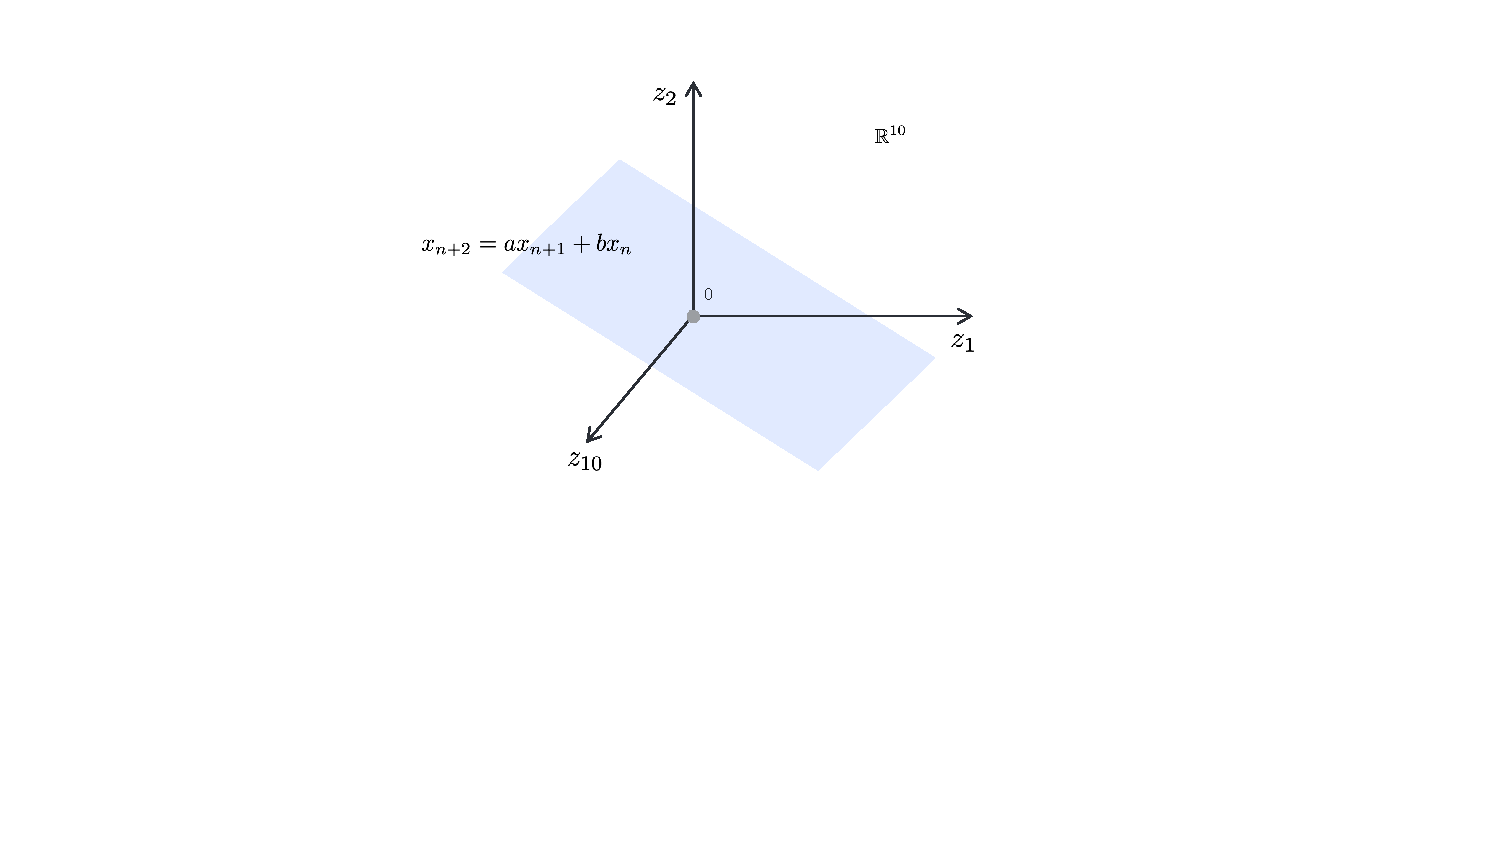
\includegraphics[width=0.6\linewidth]{\toplevelprefix/chapters/chapter1/figs/two-dimensional plane in R10.pdf}
    \caption{A two-dimensional subspace in a ten-dimensional ambient space.}
    \label{fig:lowdimplane}
\end{figure}
In practice, if we choose the segment length \(D\) large enough, all segments sampled from the same predicting function lie on a surface with intrinsic dimension \(d\), significantly lower than that of the ambient space \(D\). For example, if the sequence is given by the linear autoregression
\begin{equation}
    x_{n+2} = a x_{n+1} + b x_{n},
    \label{eqn:sequence-2d}
\end{equation}
for some constants \(a, b \in \R\), and we sample segments of length \(D = 10\), then all samples lie on a two-dimensional plane in \(\R^{10}\), as illustrated in \Cref{fig:lowdimplane}. Identifying this two-dimensional subspace fully determines the constants \(a\) and \(b\) in \eqref{eqn:sequence-2d}.

More generally, when the predicting function \(f\) is linear, as in the systems given in \eqref{eqn:lineary-system} and \eqref{eqn:lineary-system-closed}, the long segments always lie on a low-dimensional linear subspace. Identifying the predicting function is then largely equivalent to identifying this subspace, a problem known as principal component analysis. We will discuss such classic models and methods in \Cref{ch:classic}.

This observation extends to general predictable sequences: if we can identify the low-dimensional surface on which the segment samples lie, we can identify the predictive function \(f\).\footnote{Under mild conditions, there is a one-to-one mapping between the low-dimensional surface and the function \(f\). This fact has been exploited in problems such as system identification, which we will discuss later.} We cannot overemphasize the importance of this property: \textit{All samples of long segments of a predictable sequence lie on a low-dimensional submanifold.} As we will see in this book, all modern learning methods exploit this property, implicitly or explicitly.

In real-world scenarios, observed data often come from multiple predictable sequences. For example, a video sequence may contain several moving objects. In such cases, the data lie on a mixture of low-dimensional linear subspaces or nonlinear submanifolds, as illustrated in \Cref{fig:mixture-models}. 
\begin{figure}
    \centering
    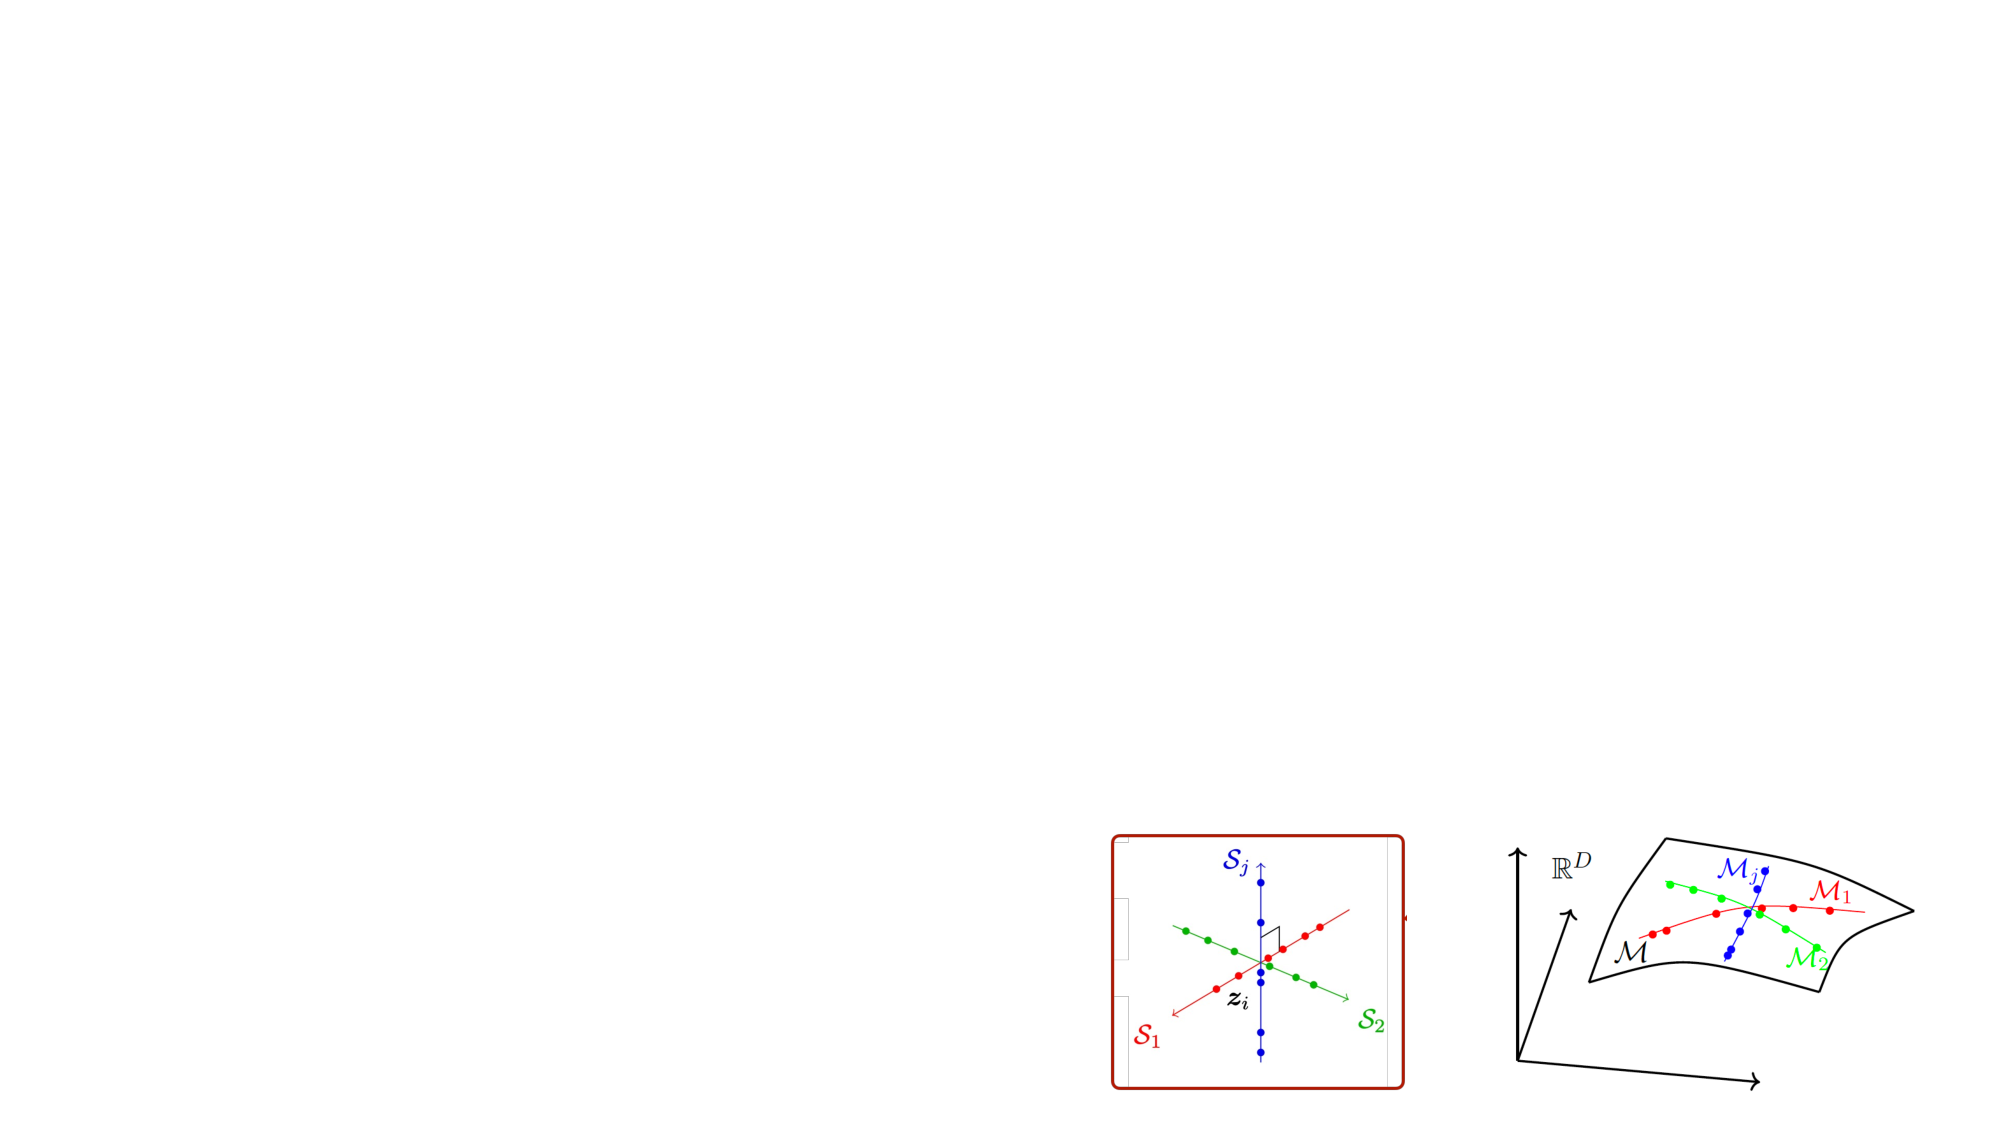
\includegraphics[width=0.8\linewidth]{\toplevelprefix/chapters/chapter1/figs/mixture.pdf}
    \caption{Data distributed on a mixture of (orthogonal) subspaces (left) or submanifolds (right).}
    \label{fig:mixture-models}
\end{figure}


\paragraph{Properties of low-dimensionality.}
Temporal correlation in predictable sequences is not the only reason data are low-dimensional. For example, the space of all images is vast, yet most of it consists of structureless random images, as shown in \Cref{fig:noise-image} (left). Natural images and videos, however, are highly redundant because of strong spatial and temporal correlations among pixel values. This redundancy allows us to recognize easily whether an image is noisy or clean, as shown in \Cref{fig:noise-image} (middle and right). Consequently, the distribution of natural images has a very low intrinsic dimension relative to the total number of pixels.

\begin{figure}
    \centering
    
\includegraphics[height=0.30\linewidth]{\toplevelprefix/chapters/chapter1/figs/Gaussian-noise.png}\hspace{2mm} 
    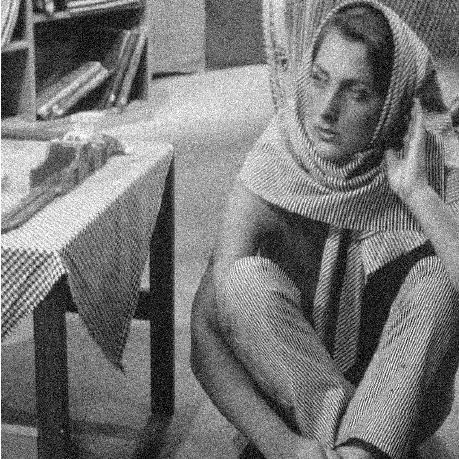
\includegraphics[height=0.30\linewidth]{\toplevelprefix/chapters/chapter1/figs/Standard-test-image-Barbara-of-size-512-512-pixels-including-Gaussian-noise-with.png} \hspace{2mm} 
    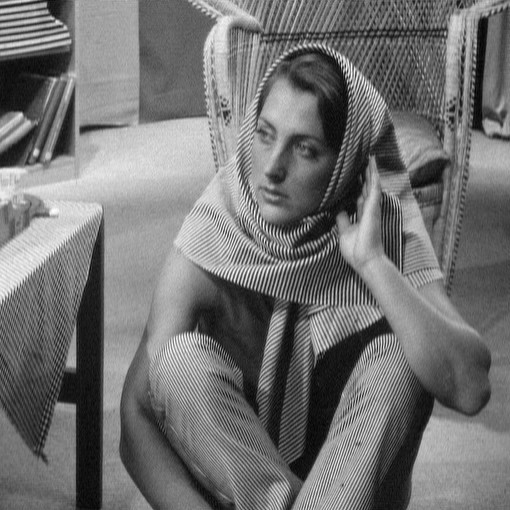
\includegraphics[height=0.30\linewidth]{\toplevelprefix/chapters/chapter1/figs/barbara.jpg}
    \caption{An image of random noise (left) versus a noisy image (middle) and the original clean image (right).}
    \label{fig:noise-image}
\end{figure}

Because learning low-dimensional structures is both important and ubiquitous, the book \textit{High-Dimensional Data Analysis with Low-Dimensional Models: Principles, Computation, and Applications} \cite{Wright-Ma-2022} begins with the statement: ``\textit{The problem of identifying the low-dimensional structure of signals or data in high-dimensional spaces is one of the most fundamental problems that, through a long history, interweaves many engineering and mathematical fields such as system theory, signal processing, pattern recognition, machine learning, and statistics.}''

By constraining the observed data point $\vx$ to lie on a low-dimensional surface, we make its entries highly dependent on one another and, in a sense, ``predictable'' from the values of other entries. For example, if we know the data are constrained to a $d$-dimensional surface in $\R^D$, we can perform several useful tasks beyond prediction:
\begin{itemize}
    \item \textbf{completion}: given more than $d$ entries of a typical sample $\vx$, the remaining entries can usually be uniquely determined;\footnote{Prediction becomes a special case of this property.}
    \item \textbf{denoising}: if the entries of a sample $\vx$ are perturbed by small noise, the noise can be effectively removed by projecting $\vx$ back onto the surface;
    \item \textbf{error correction}: if a small number of unknown entries of $\vx$ are arbitrarily corrupted, they can be efficiently corrected.
\end{itemize}
\Cref{fig:low-dim-properties} illustrates these properties using a low-dimensional linear structure---a one-dimensional line in a two-dimensional plane.

\begin{figure}
    \centering
    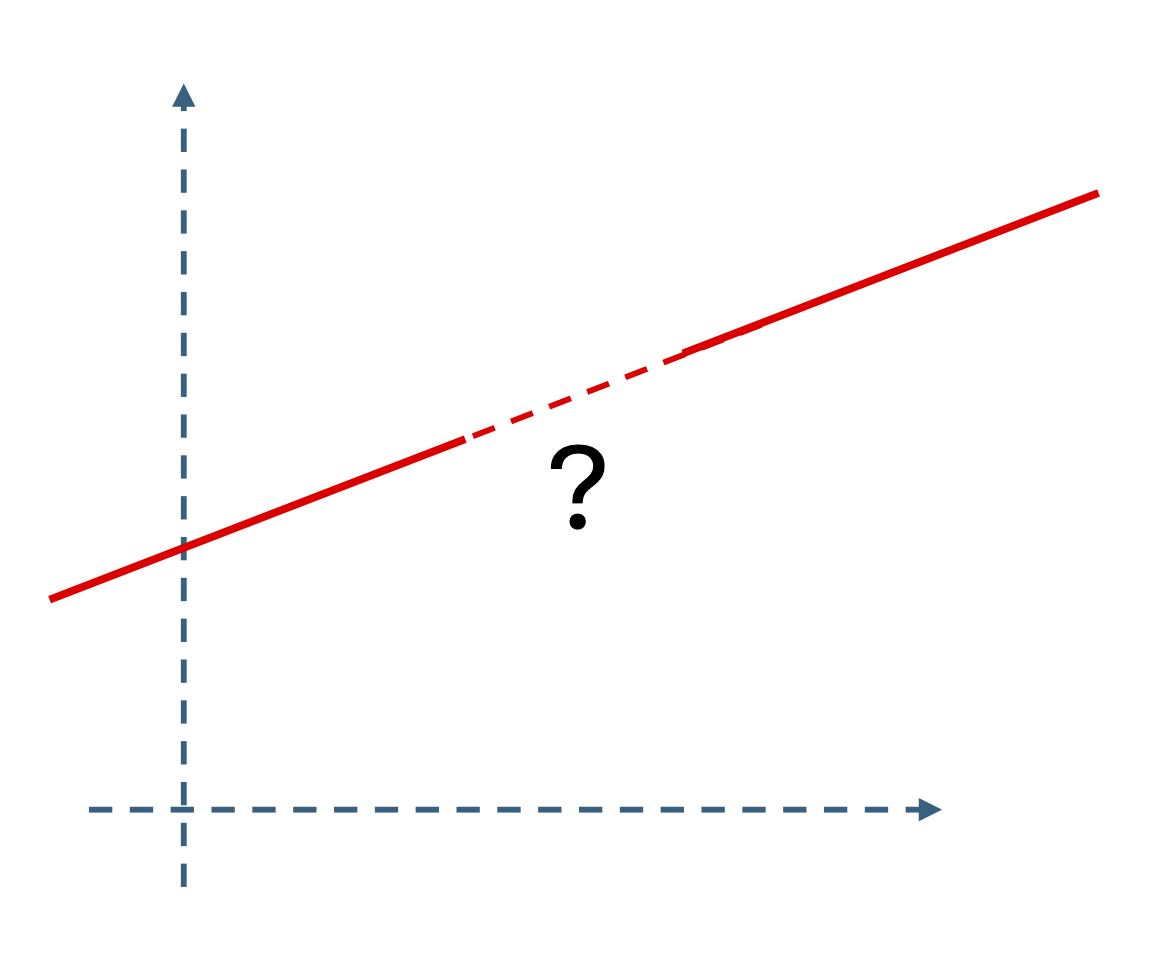
\includegraphics[height=0.28\linewidth]{\toplevelprefix/chapters/chapter1/figs/Completion-low-dim.png}     
    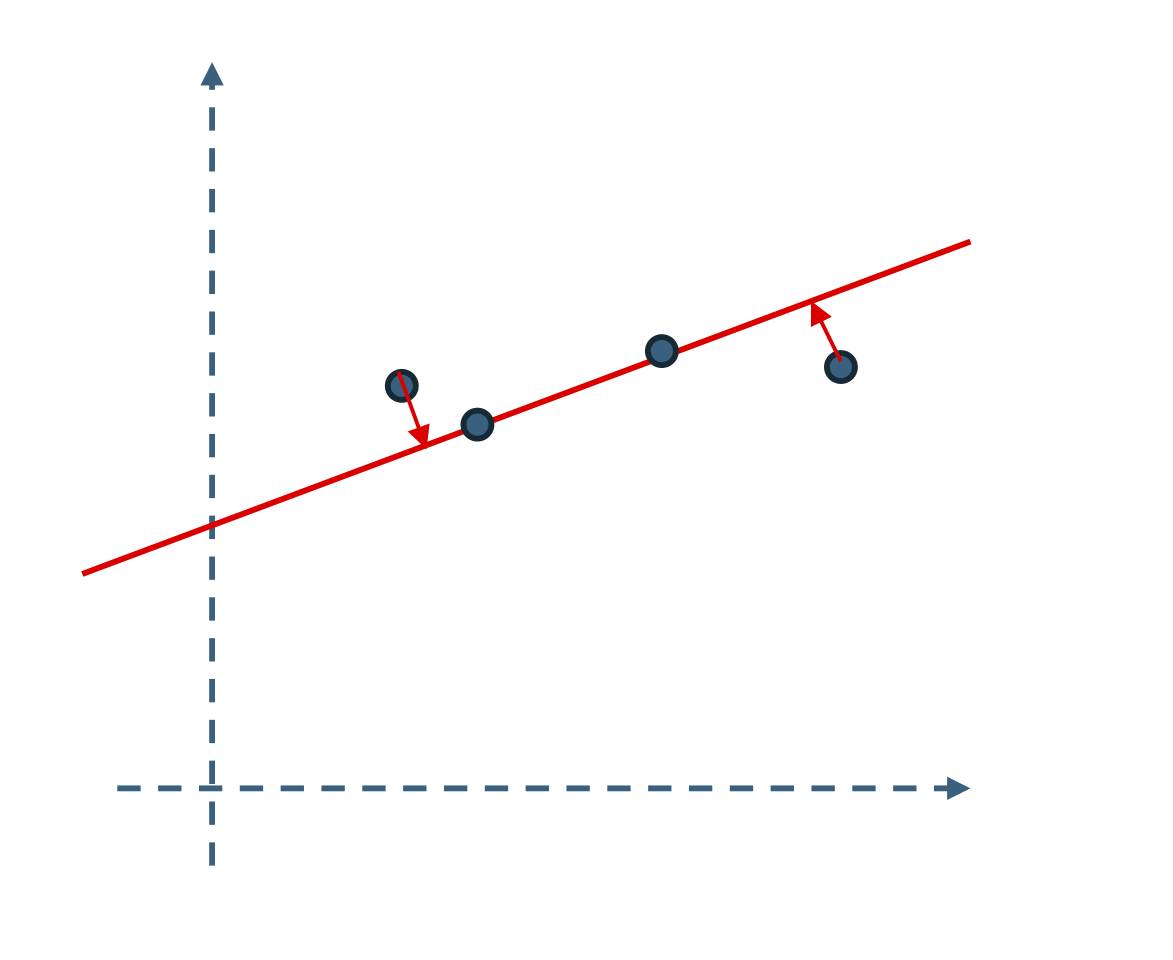
\includegraphics[height=0.28\linewidth]{\toplevelprefix/chapters/chapter1/figs/Denoising-low-dim.png} 
    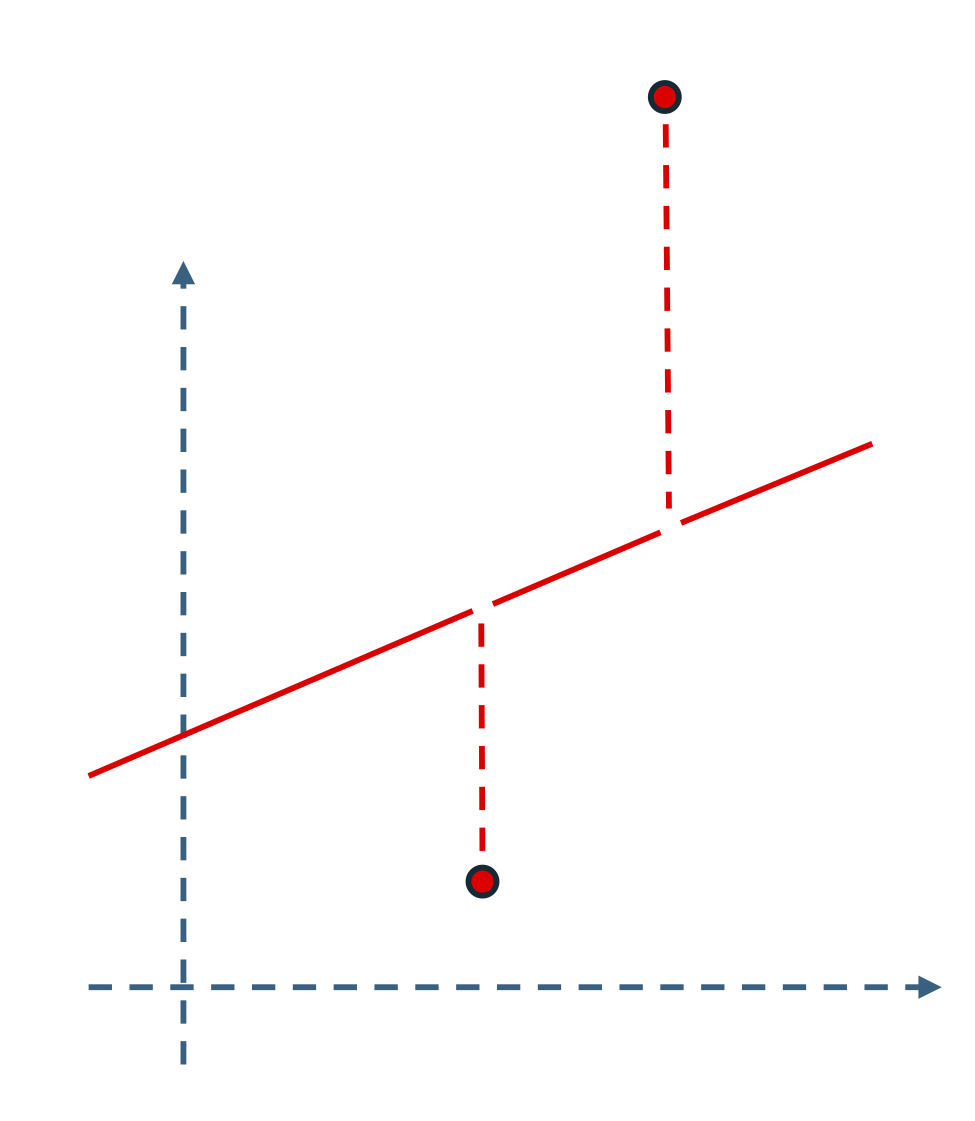
\includegraphics[height=0.32\linewidth]{\toplevelprefix/chapters/chapter1/figs/Correction-low-dim.png} 
    \caption{Illustration of properties of a low-dimensional (linear) structure: it enables completion (left), denoising (middle), and error correction (right).}
    \label{fig:low-dim-properties}
\end{figure}

Under mild conditions, these properties generalize to many other low-dimensional structures in high-dimensional spaces \cite{Wright-Ma-2022}. As we will see, these useful properties---completion and denoising, for example---inspire effective methods for learning such structures.

For simplicity, we have so far used the deterministic case to introduce the notions of predictability and low-dimensionality, where data lie precisely on geometric structures such as subspaces or surfaces. In practice, however, data always contain some uncertainty or randomness. In this case, we may assume the data follow a probability distribution with density \(p(\vx)\). A distribution is considered ``low-dimensional'' if its density concentrates around a low-dimensional geometric structure---a subspace, a surface, or a mixture thereof---as shown in \Cref{fig:mixture-models}. Once learned, such a density \(p(\vx)\) serves as a powerful prior for estimating \(\vx\) from partial, noisy, or corrupted observations:
\begin{equation}
    \vy = f(\vx) + \vn,
    \label{eqn:noisy-observation}
\end{equation}
by computing the conditional estimate \(\hat{\vx}(\vy) = \Ex(\vx \mid \vy)\) or by sampling the conditional distribution \(\hat{\vx}(\vy) \sim p(\vx\mid \vy)\).\footnote{Modern generative AI technologies, such as conditioned image generation, rely heavily on this principle, as we will discuss in \Cref{ch:conditional-inference}.}

These discussions lead to the single assumption on which this book bases its deductive approach to understanding intelligence and deep networks:
\begin{quote}
\textbf{The main assumption:} \textit{Any intelligent system or learning method should (and can) rely on the predictability of the world; hence, the distribution of observed high-dimensional data samples has low-dimensional support.}
\end{quote}
The remaining question is how to learn these low-dimensional structures correctly and computationally efficiently from high-dimensional data. As we will see, parametric models studied in classical analytical approaches and non-parametric models such as deep networks, popular in modern practice, are simply different means to the same end.

\section{How to Learn?}


\subsection{Analytical Approaches}
\label{sec:analytical}
Note that even if a predictive function is tractable to compute, it does not imply that it is tractable or scalable to learn this function from a finite number of sampled segments. One classical approach to ensure tractability is to make explicit assumptions about the family of low-dimensional structures we are dealing with. Historically, due to limited computation and data, simple and idealistic analytical models were the first to be studied, as they often offer efficient closed-form or numerical solutions. In addition, they provide insights into more general problems and already yield useful solutions to important, though limited, cases. In the old days, when computational resources were scarce, analytical models that permitted efficient closed-form or numerical solutions were the only cases that could be implemented. \textit{Linear structures} became the first class of models to be thoroughly studied.

For example, arguably the simplest case is to assume the data are distributed around a single low-dimensional subspace in a high-dimensional space. Somewhat equivalently, one may assume the data are distributed according to an almost degenerate low-dimensional Gaussian. Identifying such a subspace or Gaussian from a finite number of (noisy) samples is the classical problem of principal component analysis (PCA), and effective algorithms have been developed for this class of models \cite{JolliffeI2002}. One can make the family of models increasingly more complex and expressive. For instance, one may assume the data are distributed around a mixture of low-dimensional components (subspaces or low-dimensional Gaussians), as in independent component analysis (ICA) \cite{Ans-1985}, dictionary learning (DL), generalized principal component analysis (GPCA) \cite{Vidal-GPCA}, or the more general class of sparse low-dimensional models that have been studied extensively in recent years in fields such as compressive sensing \cite{Wright-Ma-2022}.

Across all these analytical model families, the central problem is to identify the most compact model within each family that best fits the given data. Below, we give a brief account of these classical analytical models but leave a more systematic study to \Cref{ch:classic}. In theory, these analytical models have provided tremendous insights into the geometric and statistical properties of low-dimensional structures. They often yield closed-form solutions or efficient and scalable algorithms, which are very useful for data whose distributions can be well approximated by such models. More importantly, for more general problems, they provide a sense of how easy or difficult the problem of identifying low-dimensional structures can be and what the basic ideas are to approach such a problem.


\subsubsection{Linear Dynamical Systems}
\label{sec:linear-systems}

\paragraph{Wiener filter.}

As discussed in \Cref{sec:predictability}, a central task of intelligence is to learn what is predictable in sequences of observations. The simplest class of predictable sequences---or signals---are those generated by a \textit{linear time-invariant} (LTI) process:
\begin{equation}
    x[n] = h[n]*z[n] + \epsilon[n], 
    \label{eqn:Wiener-model}
\end{equation}
where \(*\) is the convolution operation, \(z\) is the input and \(h\) is the impulse response function.\footnote{Typically, \(h\) is assumed to have certain desirable properties, such as finite length or a band-limited spectrum.} Here \(\epsilon[n]\) denotes additive observation noise. Given the input process \(\{z[n]\}\) and observations of the output process \(\{x[n]\}\), the goal is to find the optimal \(h[n]\) such that \(\hat{x}[n] = h[n]*z[n]\) predicts \(x[n]\) optimally. Prediction quality (i.e., goodness) is measured by the mean squared error (MSE):
\begin{equation}
    \min_{h} \Ex[\epsilon[n]^{2}] = \Ex[\|x[n] - h[n]*z[n]\|_{2}^{2}].
    \label{eqn:wiener-mse}
\end{equation}
The optimal solution \(h[n]\) is called a (denoising) filter. Norbert Wiener---who also initiated the Cybernetics movement---studied this problem in the 1940s and derived an elegant closed-form solution known as the \textit{Wiener filter} \cite{Wiener-1942,Wiener-1949}. This result, also known as least-variance estimation and filtering, became one of the cornerstones of signal processing. Interested readers may refer to \cite[Appendix B]{MaY2003} for a detailed derivation of this type of estimator.

\paragraph{Kalman filter.} 
The idea of denoising or filtering a dynamical system was later extended by Rudolph Kalman in the 1960s to a linear time-invariant system described by a finite-dimensional state-space model:
\begin{equation}
    \vz[n] = \vA \vz[n-1] + \vB\vu[n] + \vepsilon[n]. 
    \label{eqn:linear-state-space}
\end{equation}
The problem is to estimate the system state \(\vz[n]\) from noisy observations of the form
\begin{equation}
    \vx[n] = \vC \vz[n] + \vw[n],
    \label{eqn:Kalman-model}
\end{equation}
where \(\vw\) is (white) noise. The optimal causal\footnote{This means the estimator can use only observations up to the current time step \(n\). The Kalman filter is always causal, whereas the Wiener filter need not be.} state estimator that minimizes the minimum-MSE (MMSE) prediction error
\begin{equation}
    \min \Ex[ \|\vx[n] - \vC\vz[n]\|_{2}^{2}]
    \label{eqn:kalman-mse}
\end{equation}
is given in closed form by the so-called \textit{Kalman filter} \cite{kalman1960new}. This result is a cornerstone of modern control theory because it enables estimation of a dynamical system's state from noisy observations. One can then introduce linear state feedback, for example \(\vu[n] = \vF \hat{\vz}[n]\), and render the closed-loop system fully autonomous, as shown in \Cref{eqn:recursive-closed-loop}.  Interested readers may refer to \cite[Appendix B]{MaY2003} for a detailed derivation of the Kalman filter.

\paragraph{Identification of linear dynamical systems.}
To derive the Kalman filter, the system parameters \(\vA, \vB, \vC\) are assumed to be known. If they are not given in advance, the problem becomes more challenging and is known as \textit{system identification}: how to \textit{learn} the parameters \(\vA, \vB, \vC\) from many samples of the input sequence \(\{\vu[n]\}\) and observation sequence \(\{\vx[n]\}\). This is a classic problem in systems theory. If the system is linear, the input and output sequences \(\{\vu[n], \vx[n]\}\) jointly lie on a certain low-dimensional subspace\footnote{which has the same dimension as the order of the state-space model \eqref{eqn:linear-state-space}.}. Hence, the identification problem is essentially equivalent to identifying this low-dimensional subspace \cite{OverscheeP1996,Liu-2009-CDC,Liu-2010-SIAM}.

Note that the above problems have two things in common: first, the noise-free sequences or signals are assumed to be generated by an explicit family of parametric models; second, these models are essentially linear. Conceptually, let \(\vx_{o}\) be a random variable whose ``true'' distribution is supported on a low-dimensional linear subspace, say \(S\). To a large extent, the Wiener filter and Kalman filter both try to estimate such an \(\vx_{o}\) from its noisy observations:
\begin{equation}
    \vx = \vx_{o} + \vepsilon, \quad \vx_{o} \sim S,
\end{equation}
where \(\vepsilon\) is typically a random Gaussian noise (or process). Hence, their solutions rely on identifying a low-dimensional linear subspace that best fits the observed noisy data. By projecting the data onto this subspace, one obtains the optimal denoising operations, all in closed form.


\subsubsection{Linear and Mixed Linear Models}
\label{sec:PCA-ICA}
\paragraph{Principal component analysis.}
From the above problems in classical signal processing and system identification, we see that the main task behind all these problems is to learn a \textit{single} low-dimensional linear subspace from noisy observations. Mathematically, we may model such a structure as
\begin{equation}
    \vx = \vu_{1} z_{1} + \vu_{2} z_{2} + \cdots + \vu_{d} z_{d} + \vepsilon =  \vU \vz + \vepsilon, \quad \vU \in \R^{D\times d},
    \label{eqn:PCA-model}
\end{equation}
where \(\vepsilon \in \R^{D}\) is small random noise. \Cref{fig:PCA} illustrates such a distribution with two principal components.
\begin{figure}
    \centering
    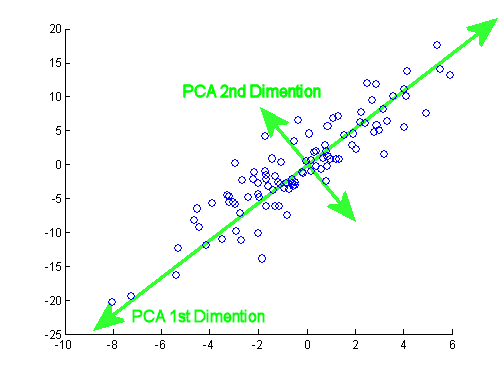
\includegraphics[width=0.5\linewidth]{\toplevelprefix/chapters/chapter1/figs/PCA.png}
    \caption{A distribution with two principal components.}
    \label{fig:PCA}
\end{figure}
The problem is to find the subspace basis \(\vU\) from many samples of \(\vx\). A typical approach is to minimize the projection error onto the subspace:
\begin{equation}
    \min_{\vU}\Ex[\|\vx - \vU\vU^{\top} \vz\|_{2}^{2}].
\end{equation}
This is essentially a denoising task: once the basis \(\vU\) is correctly found, we can denoise the noisy sample \(\vx\) by projecting it onto the low-dimensional subspace spanned by \(\vU\):
\begin{equation}
\vx \rightarrow \hat{\vx} = \vU\vU^{\top} \vx. 
\end{equation}
If the noise is small and the low-dimensional subspace \(\vU\) is correctly learned, we expect \(\vx \approx \hat{\vx}\). Thus, PCA is a special case of a so-called ``auto-encoding'' scheme, which encodes the data by projecting it into a lower-dimensional space, and decodes a lower-dimensional code by it into the original space:
\begin{equation}
    \vx   \xrightarrow{\hspace{2mm} \vU^{\top}\hspace{2mm}} \vz  \xrightarrow{\hspace{2mm} \vU \hspace{2mm}} \hat{\vx}.
       \label{eqn:auto-encoding-PCA}
\end{equation}
Because of the simple data structure, the encoder \(\cE\) and decoder \(\cD\) both become simple linear operators (projecting and lifting).

This classic problem in statistics is known as principal component analysis (PCA). It was first studied by Pearson in 1901 \cite{Pearson1901} and later independently by Hotelling in 1933 \cite{Hotelling1933}. The topic is systematically summarized in the classic book \cite{Jolliffe1986,JolliffeI2002}.
One may also explicitly assume the data \(\vx\) is distributed according to a single low-dimensional Gaussian:
\begin{equation}
    \vx \sim \mathcal{N}(\vzero, \vU\vU^{\top} + \sigma \vI), \quad \vU \in \R^{D\times d},
\end{equation}
which is equivalent to assuming that \(\vz\) in the PCA model \eqref{eqn:PCA-model} is a standard normal distribution. This problem is known as probabilistic PCA \cite{TippingM1999} and has the same computational solution as PCA. 

In this book, we revisit PCA in \Cref{ch:classic} from the perspective of learning a low-dimensional distribution. Our goal is to use this simple and idealistic model to convey some of the most fundamental ideas for learning a compact representation of a low-dimensional distribution, including the important notions of compression via denoising and auto-encoding for a consistent representation.
\paragraph{Independent component analysis.}
Independent component analysis (ICA) was originally proposed by \cite{Ans-1985} as a classic model for \textit{learning a good representation}. In fact, it was originally proposed as a simple mathematical model for our memory. The ICA model takes a deceptively similar form to the above PCA model \eqref{eqn:PCA-model} by assuming that the observed random variable \(\vx\) is a linear superposition of multiple independent components \(z_{i}\):\footnote{In PCA the ``components'' are the learned vectors, whereas in ICA they are scalars. This is just a difference in names and convention.}
\begin{equation}
    \vx = \vu_{1} z_{1} + \vu_{2} z_{2} + \cdots + \vu_{d} z_{d}  + \vepsilon =  \vU \vz + \vepsilon.
    \label{eqn:ICA-model}
\end{equation}
However, here the components \(z_{i}\) are assumed to be independent \textit{non-Gaussian} variables. For example, a popular choice is
\begin{equation}
    z_{i} = \sigma_{i} \cdot w_{i}, \quad \sigma_{i} \sim B(1,p),
    \label{eqn:ICA-modes}
\end{equation}
where \(\sigma_{i}\) is a Bernoulli random variable and \(w_{i}\) could be a constant value or another random variable, say Gaussian.\footnote{Even if \(w\) is Gaussian, \(\sigma w\) is no longer a Gaussian variable!} The ICA problem aims to identify both \(\vU\) and \(\vz\) from observed samples of \(\vx\). \Cref{fig:ICA-PCA} illustrates the difference between ICA and PCA.

\begin{figure}
    \centering
    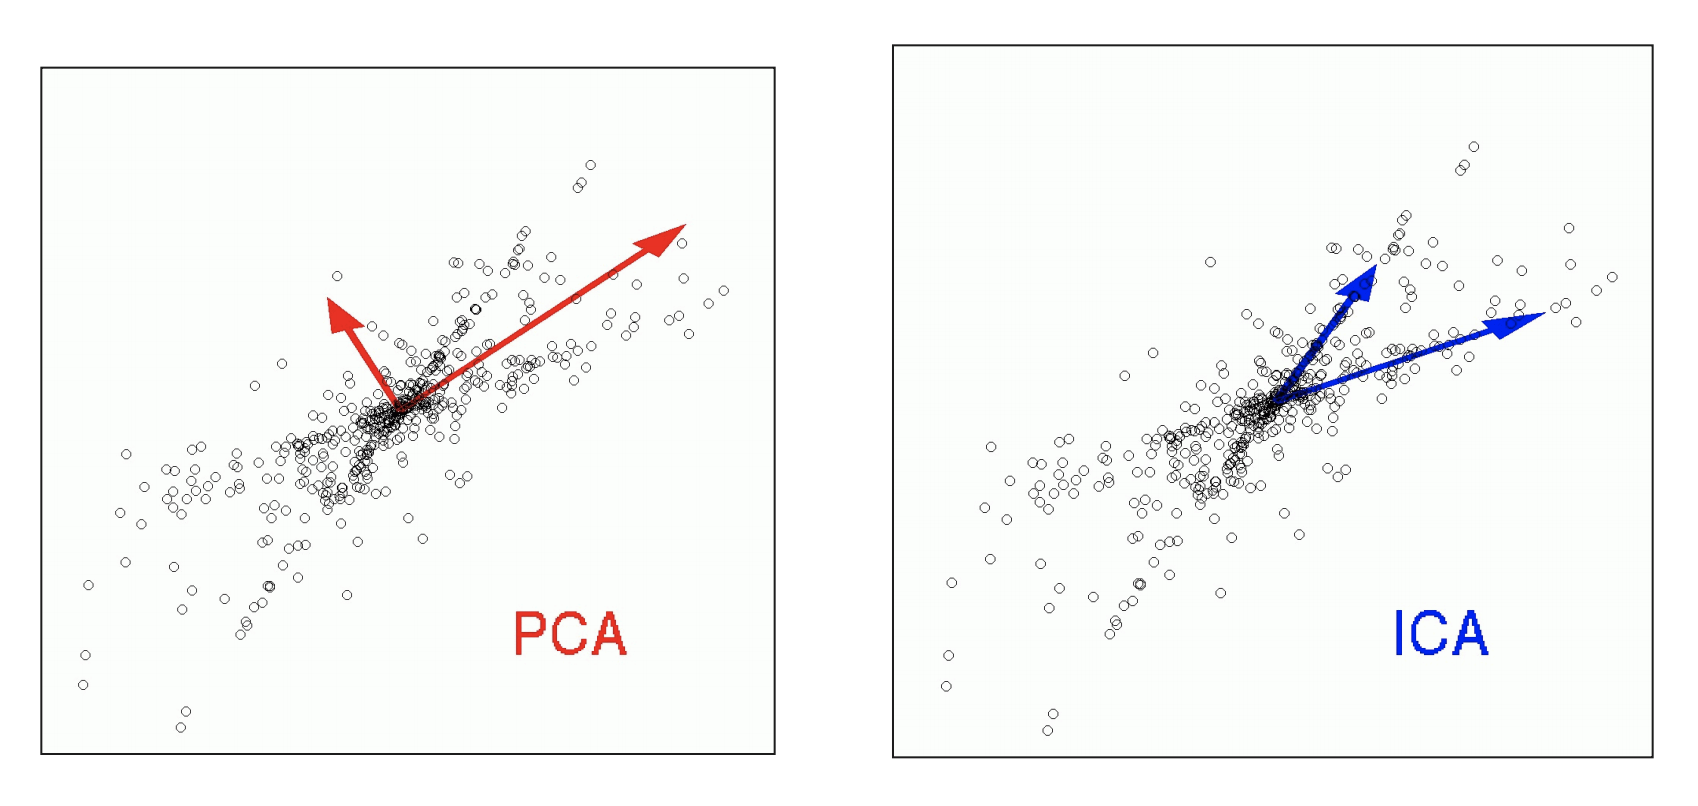
\includegraphics[width=0.7\linewidth]{\toplevelprefix/chapters/chapter1/figs/PCA_ICA.png}
    \caption{PCA (left) versus ICA (right). Note that PCA finds the \textit{orthogonal} vectors that approximately span the data, while ICA finds (not necessarily orthogonal) vectors that \textit{independently} combine to approximately form the data, as well as the coefficients of this combination.}
    \label{fig:ICA-PCA}
\end{figure}

Although the (decoding) mapping from \(\vz\) to \(\vx\) seems linear and straightforward once \(\vU\) and \(\vz\) are learned, the (encoding) mapping from \(\vx\) to \(\vz\) can be complicated and may not be represented by a simple linear mapping. Hence, ICA generally gives an auto-encoding of the form:
\begin{equation}
    \vx   \xrightarrow{\hspace{2mm} \cE\hspace{2mm}} \vz  \xrightarrow{\hspace{2mm} \vU \hspace{2mm}} \hat{\vx}.
       \label{eqn:auto-encoding-ICA}
\end{equation}
Thus, unlike PCA, ICA is somewhat more difficult to analyze and solve. In the 1990s, researchers such as Erkki Oja and Aapo Hyv\"{a}rinen \cite{hyvarinen-1997,Hyvrinen-2000} made significant theoretical and algorithmic contributions to ICA. In \Cref{ch:classic}, we will study and provide a solution to ICA from which the encoding mapping \(\cE\) will become clear.


\paragraph{Sparse structures and compressive sensing.}
If \(p\) in \eqref{eqn:ICA-modes} is very small, the probability that any component is non-zero is small. In this case we say \(\vx\) is sparsely generated and concentrates on a union of linear subspaces whose dimension is \(k = p \cdot d\). We may therefore extend the ICA model to a more general family of low-dimensional structures known as sparse models.

A \(k\)-sparse model is the set of all \textit{\(k\)-sparse vectors}:
\begin{equation}
    \cZ = \{\vz \in \R^{n} \mid \|\vz\|_{0} \leq k\},
\end{equation}
where \(\|\cdot\|_{0}\) counts the number of non-zero entries. Thus \(\cZ\) is the union of all \(k\)-dimensional subspaces aligned with the coordinate axes, as illustrated in \Cref{fig:mixture-models} (left). A central problem in signal processing and statistics is to recover a sparse vector \(\vz\) from its linear observations
\begin{equation}
    \vx = \vA \vz + \vepsilon, \quad \vA \in \R^{m\times n},
    \label{eqn:sparse-model}
\end{equation}
where \(\vA\) is given, typically \(m < n\), and \(\vepsilon\) is small noise. This seemingly benign problem is NP-hard to solve and even hard to approximate (see \cite{Wright-Ma-2022} for details).

Despite a rich history dating back to the eighteenth century \cite{Boscovichca1750}, no provably efficient algorithm existed for this class of problems, although many heuristic algorithms were proposed between the 1960s and 1990s. Some were effective in practice but lacked rigorous justification. A major breakthrough came in the early 2000s when mathematicians including David Donoho, Emmanuel Cand\'{e}s, and Terence Tao \cite{donoho2005neighborly,Candes2005,CandesE2005-IT} established a rigorous theoretical framework that characterizes precise conditions under which the sparse recovery problem can be solved effectively and efficiently via convex \(\ell^{1}\) minimization:
\begin{equation}
    \min \|\vz\|_{1} \quad \text{subject to} \quad \|\vx - \vA\vz\|_{2} \leq \epsilon,
\end{equation}
where \(\|\cdot\|_{1}\) is the sparsity-promoting \(\ell^{1}\) norm of a vector and \(\epsilon\) is a small constant. Any solution yields a sparse (auto) encoding 
\begin{equation}
    \vx \xrightarrow{\hspace{2mm} \cE \hspace{2mm}} \vz \xrightarrow{\hspace{2mm} \vA \hspace{2mm}} \hat{\vx}.
    \label{eqn:decoding-sparse}
\end{equation}
We will describe such an algorithm (and thus mapping) in \Cref{ch:classic}, revealing fundamental connections between sparse coding and deep learning.\footnote{Similarities between sparse-coding algorithms and deep networks were noted as early as 2010 \cite{gregor2010learning}.}

Conditions for \(\ell^{1}\) minimization to succeed are surprisingly general: the minimum number of measurements \(m\) required for a successful recovery is only proportional to the intrinsic dimension \(k\). This is the \textit{compressive sensing} phenomenon \cite{CandesE2006-ICM}. It extends to broad families of low-dimensional structures, including low-rank matrices. These results fundamentally changed our understanding of recovering low-dimensional structures in high-dimensional spaces. David Donoho, among others, celebrated this reversal as the ``blessing of dimensionality'' \cite{DonohoD2000}, in contrast to the usual pessimistic belief in the ``curse of dimensionality.'' The complete theory and body of results is presented in \cite{Wright-Ma-2022}.

The computational significance of this framework cannot be overstated. It transformed problems previously believed intractable into ones that are not only tractable but scalably solvable using extremely efficient algorithms:
\begin{equation}
    \text{intractable} \;\Longrightarrow\; \text{tractable} \;\Longrightarrow\; \text{scalable}.
\end{equation}
The algorithms come with rigorous theoretical guarantees of correctness given precise requirements in data and computation. The deductive nature of this approach contrasts sharply with the empirical, inductive practice of deep neural networks. Yet we now know that both approaches share a common goal---pursuing low-dimensional structures in high-dimensional spaces.

\paragraph{Dictionary learning.}
Conceptually, an even harder problem than the sparse-coding problem \eqref{eqn:sparse-model} arises when the observation matrix \(\vA\) is unknown and must itself be learned from a set of (possibly noisy) observations \(\vX = [\vx_{1}, \vx_{2}, \ldots, \vx_{n}]\):
\begin{equation}
    \vX = \vA \vZ + \vE, \quad \vA \in \R^{m\times n}.
    \label{eqn:dictionary-learning}
\end{equation}
Here we are given only \(\vX\), not the corresponding \(\vZ = [\vz_{1}, \vz_{2}, \ldots, \vz_{n}]\) or the noise term \(\vE = [\vepsilon_{1}, \vepsilon_{2}, \ldots, \vepsilon_{n}]\), except that the \(\vz_{i}\) are known to be sparse. This is the \textit{dictionary learning} problem, which generalizes the ICA problem \eqref{eqn:ICA-model} discussed earlier. In other words, given that the distribution of the data \(\vX\) is the image of a standard sparse distribution \(\vZ\) under a linear transform \(\vA\), we wish to learn both \(\vA\) and its ``inverse'' mapping \(\cE\) so as to obtain an autoencoder:
\begin{equation}
    \vX   \xrightarrow{\hspace{2mm} \cE\hspace{2mm}}  \vZ \xrightarrow{\hspace{2mm} \vA \hspace{2mm}} \hat{\vX}.
       \label{eqn:decoding-DL}
\end{equation}

PCA, ICA, and dictionary learning all assume that the data distribution is supported on or near low-dimensional linear or piecewise-linear structures. Each method requires learning a (global or local) basis for these structures from noisy samples. In \Cref{ch:classic} we study how to identify such low-dimensional structures through these classical models. In particular, we will see that all of these low-dimensional (piecewise) linear models can be learned efficiently by the same family of fast algorithms known as \textit{power iteration} \cite{Zhai-2020}. Although these linear or piecewise-linear models are somewhat idealized for most real-world data, understanding them is an essential first step toward understanding more general low-dimensional distributions.

\subsubsection{General Distributions}\label{sec:denoising-intro}

The distributions of real-world data such as images, videos, and audio are too complex to be modeled by the above, somewhat idealistic, linear models or Gaussian processes. We normally do not know \textit{a priori} from which family of parametric models they are generated. Historically, many attempts have been made to develop analytical models for these data. In particular, Fields Medalist David Mumford spent considerable effort in the 1990s trying to understand and model the statistics of natural images \cite{Mumford1996TheSD}. He and his students, including Song-Chun Zhu, drew inspiration and techniques from statistical physics and proposed many statistical and stochastic models for the distribution of natural images, such as random fields or stochastic processes \cite{Zhu-Entropy-1997,Zhu1997LearningGP,Zhu1997Prior,Huang-Mumford,Mumford-1999,Lee-Mumford}. However, these analytical models achieved only limited success in producing samples that closely resemble natural images. Clearly, for real-world data like images, we need to develop more powerful and unifying methods to pursue their more general low-dimensional structures.

In practice, for a general distribution of real-world data, we typically only have many samples from the distribution---the so-called \textit{empirical distribution}. In such cases, we normally cannot expect to have a clear analytical form for their low-dimensional structures, nor for the resulting denoising operators.\footnote{This is unlike the cases of PCA, Wiener filter, and Kalman filter.} We therefore need to develop a more general solution to these empirical distributions, not necessarily in closed form but at least efficiently computable. If we do this correctly, solutions to the aforementioned linear models should become their special cases.

\paragraph{Denoising.} In the 1950s, statisticians became interested in the problem of denoising data drawn from an arbitrary distribution. Let \(\vx_{o}\) be a random variable with probability density function \(p_{o}(\cdot)\). Suppose we observe a noisy version of \(\vx_{o}\):
\begin{equation}
    \vx = \vx_{o} + \sigma \vg, 
\end{equation}
where \(\vg \sim \dNorm(\vzero, \vI)\) is standard Gaussian noise and \(\sigma\) is the noise level of the observation. Let \(p(\cdot)\) be the probability density function of \(\vx\).\footnote{That is, \(p(\vx) = \int_{-\infty}^{\infty} \phi_{\sigma}(\vx - \vz)p_{o}(\vz) \odif{\vz}\), where \(\phi_{\sigma}\) is the density function of the Gaussian distribution \(\mathcal{N}(\vzero, \sigma^{2} \vI)\).} Remarkably, the posterior expectation of \(\vx_{o}\) given \(\vx\) can be calculated by an elegant formula, known as Tweedie's formula \cite{Robbins1956AnEB}:\footnote{Herbert Robbins gave the credit for this formula to Maurice Kenneth Tweedie from their personal correspondence.}
\begin{equation}
    \hat{\vx}_{o} = \Ex[\vx_{o}\mid \vx] = \vx + \sigma^{2} \nabla \log p(\vx).
\end{equation}
As can be seen from the formula, the function \(\nabla \log p(\vx)\) plays a very special role in denoising the observation \(\vx\) here. The noise \(\vg\) can be explicitly estimated as
\begin{equation}
    \hat{\vg} = \frac{\vx - \hat{\vx}_{o}}{\sigma} = -\sigma \nabla \log p(\vx),
\end{equation}
for which we only need to know the distribution \(p(\cdot)\) of \(\vx\), not the ground truth \(p_{o}(\cdot)\) for \(\vx_{o}\). An important implication of this result is that if we add Gaussian noise to any distribution, the denoising process can be done easily if we can somehow obtain the function \(\nabla \log p(\vx)\).

Because this is such an important and useful result, it has been rediscovered and used in many different contexts and areas. For example, after Tweedie's formula \cite{Robbins1956AnEB}, it was rediscovered a few years later by \cite{Miyasawa61} where it was termed ``empirical Bayesian denoising.'' In the early 2000s, the function \(\nabla \log p(\vx)\) was rediscovered again in the context of learning a general distribution and was named the ``score function'' by Aapo Hyv\"{a}rinen \cite{hyvarinen05a}. Its connection to (empirical Bayesian) denoising was soon recognized by \cite{Vincent2011}.
Generalizations to other measurement distributions (beyond Gaussian noise) have been made by Eero Simoncelli's group \cite{Raphan10}. Today, the most direct application of Tweedie's formula and denoising is image generation via iterative denoising \cite{Kadkhodaie21a,ho2020denoising}.

\begin{figure}
    \centering
    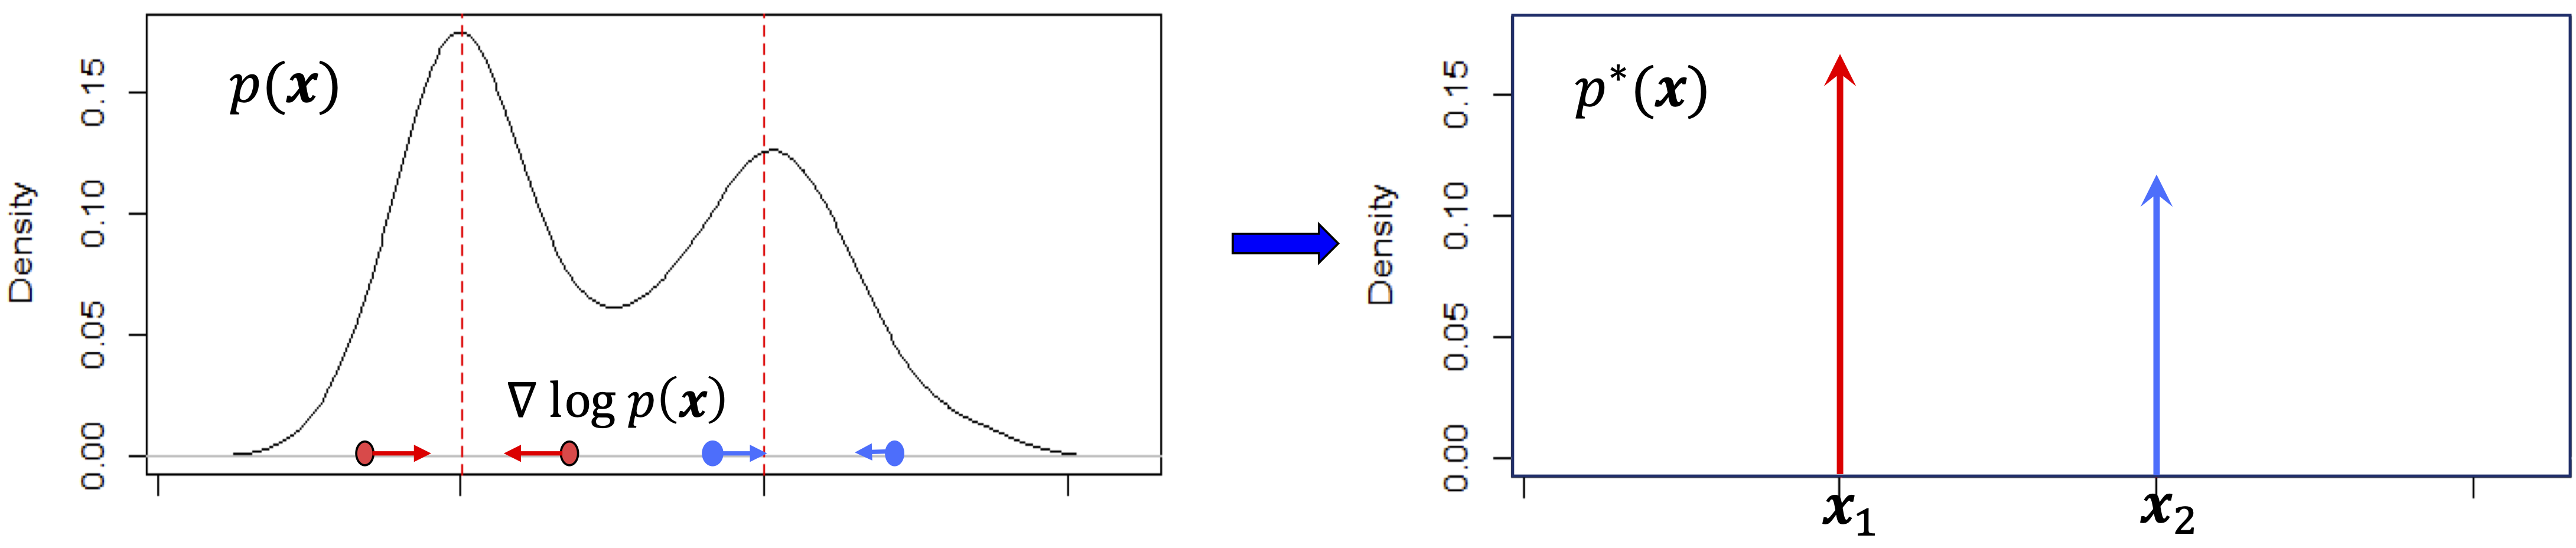
\includegraphics[width=1\linewidth]{\toplevelprefix/chapters/chapter1/figs/Density-compress.png}
    \caption{Geometric interpretation of a score function \(\nabla \log p(\vx)\) for a distribution with density \(p(\vx)\) on the left. The operation generated by the score function pushes the distribution towards areas of higher density. The goal is that, by a certain measure of compactness (e.g. entropy or coding length), the resulting distribution is more ``compressed''. Eventually, the distribution converges to one that has a lower-dimensional support, as \(p^{*}(\vx)\) shown on the right.}
    \label{fig:score-function}
\end{figure}

\paragraph{Entropy minimization.} The score has an intuitive information-theoretic and geometric interpretation. In information theory, \(-\log p(\vx)\) corresponds to the number of bits needed to encode \(\vx\)\footnote{at least for discrete variables, as detailed in \Cref{ch:compression}.}. The gradient \(\nabla \log p(\vx)\) points toward higher-probability-density regions, as shown in \Cref{fig:score-function} (left). Moving in this direction reduces the number of bits required to encode \(\vx\). Thus, the operator \(\nabla \log p(\vx)\) pushes the distribution to ``shrink'' toward high-density regions. Formally, one can show that the (differential) entropy
\begin{equation}
    H(\vx) = - \int p(\vw) \log p(\vw) \odif{\vw}
\end{equation}
decreases under this operation (see \Cref{ch:compression} and \Cref{app:diffusion-denoising}). With an optimal codebook, the resulting distribution achieves a lower coding rate and is thus more compressed. Repeating this denoising process indefinitely produces a distribution whose probability mass is concentrated on a support of lower dimension. For instance, the distribution \(p(\vx)\) in \Cref{fig:score-function} (left) converges to \(p^{*}(\vx)\) (right):\footnote{Strictly speaking, \(p^{*}(\vx)\) is a generalized function: \(p^{*}(\vx) = p^{*}(\vx_{1})\delta(\vx-\vx_{1}) + p^{*}(\vx_{2}) \delta(\vx-\vx_{2})\) with \(p^{*}(\vx_{1}) + p^{*}(\vx_{2}) = 1\).}\footnote{Notice that in this section we discuss the process of iteratively denoising and compressing a high-entropy noise distribution until it converges to the low-entropy data distribution. As we will see in \Cref{ch:general-distribution}, this problem is dual to the problem of learning an optimal encoding for the data distribution, which is also a useful application \cite{relic2024lossy}.}
\begin{equation}
    H(\vx) = - \int p(\vw) \log p(\vw) \odif{\vw} \quad \xrightarrow{\hspace{1mm} \text{decreasing} \hspace{1mm}} \quad H^{*}(\vx) = - \int p^{*}(\vw) \log p^{*}(\vw) \odif{\vw}.
\end{equation}
As the distribution converges to \(p^{*}(\vx)\), its differential entropy approaches negative infinity due to a technical difference between continuous and discrete entropy definitions. \Cref{ch:compression} resolves this using a unified \textit{rate-distortion} measure.

Later in this chapter and \Cref{ch:compression}, we explore how this simple denoising-compression framework unifies powerful methods for learning low-dimensional distributions in high-dimensional spaces, including natural image distributions.
\subsection{Empirical Approaches}
In practice, it is difficult to model important real-world data---such as images, sounds, and text---with the idealized linear, piecewise-linear, or other analytical models discussed in the previous section. Historically, many empirical models and methods have therefore been proposed. These models often drew inspiration from the biological nervous system, because the brain of an animal or human processes such data with remarkable efficiency and effectiveness.

\subsubsection{Classic Artificial Neural Networks}
\paragraph{Artificial neuron.}

\begin{figure}[t]
    \centering
    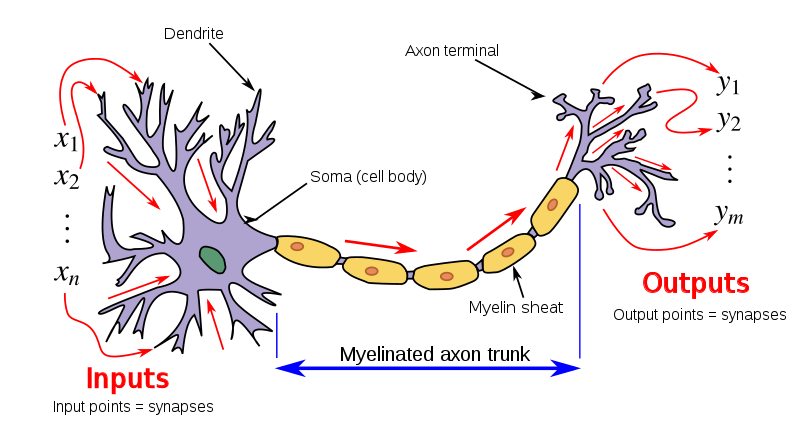
\includegraphics[width=0.55\linewidth]{\toplevelprefix/chapters/chapter1/figs/neuron.png} \hspace{3mm}   
    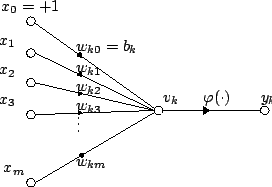
\includegraphics[width=0.40\linewidth]{\toplevelprefix/chapters/chapter1/figs/Artificial_neuron.png}
    \caption{The first mathematical model of an artificial neuron (right) that emulates how a neuron (left) processes signals.}
    \label{fig:neuron}
\end{figure}

Inspired by the nervous system in the brain, the first mathematical model of an artificial neuron\footnote{known as the Linear Threshold Unit, or perceptron.} was proposed by Warren McCulloch\footnote{a professor of psychiatry at the University of Chicago at the time} and Walter Pitts in 1943 \cite{McCulloch-Pitts}. It describes the relationship between the input $x_i$ and output $o_j$ as:
\begin{equation}
    o_j = \varphi\Big( \sum_i w_{ji}x_i\Big),  
\end{equation}
where $\varphi(\cdot)$ is some nonlinear activation, typically modeled by a threshold function. This model is illustrated in \Cref{fig:neuron}. As we can see, this form already shares the main characteristics of a basic unit in modern deep neural networks. The model is derived from observations of how a single neuron works in our nervous system. However, researchers did not know exactly what functions a collection of such neurons could realize and perform. On a more technical level, they were also unsure which nonlinear activation function $\varphi(\cdot)$ should be used. Hence, historically many variants have been proposed.\footnote{Step function, hard or soft thresholding, rectified linear unit (ReLU), sigmoid, etc. \cite{dubey2022activation}.}

\begin{figure}[t]
\centering
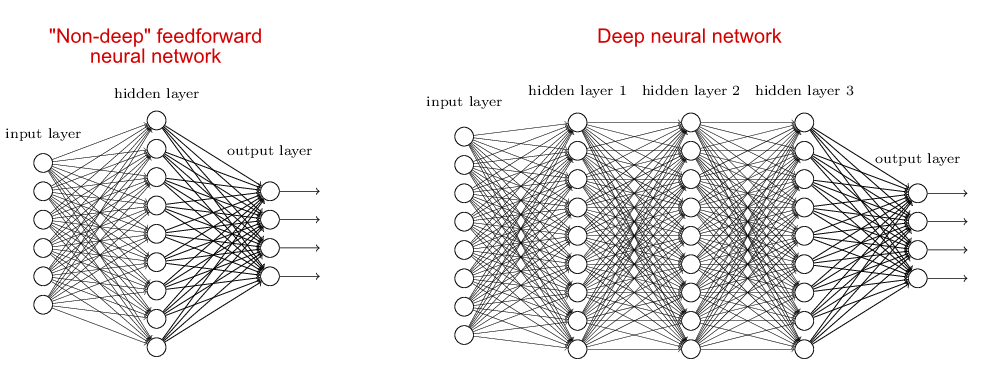
\includegraphics[width=0.85\linewidth]{\toplevelprefix/chapters/chapter1/figs/single-deep.png}
    \caption{A network with one hidden layer (left) versus a deep network (right).}
    \label{fig:single-deep}
\end{figure}

\paragraph{Artificial neural network.}
In the 1950s, Frank Rosenblatt was the first to build a machine with a \textit{network} of such artificial neurons, shown in \Cref{fig:perceptron}. The machine, called Mark I Perceptron, consists of an input layer, an output layer, and a single hidden layer of 512 artificial neurons, as shown in \Cref{fig:perceptron} left, which is similar to what is illustrated in \Cref{fig:single-deep} (left). It was designed to classify optical images of letters. However, the capacity of a single-layer network is limited and can only learn linearly separable patterns. In the 1969 book \textit{Perceptrons: An Introduction to Computational Geometry} by Marvin Minsky and Seymour Papert \cite{Minsky-1969}, it was shown that the single-layer architecture of Mark I Perceptron cannot learn an XOR function. This result significantly dampened interest in artificial neural networks, even though it was later proven that a multi-layer network can learn an XOR function \cite{Rumelhart1986}. In fact, a sufficiently large multi-layer network, as shown in \Cref{fig:single-deep} (right), consisting of such simple neurons can simulate any finite-state machine, even the universal Turing machine.\footnote{Do not confuse what neural networks are capable of doing in principle with whether it is tractable or easy to learn a neural network that realizes certain desired functions.} Nevertheless, the study of artificial neural networks subsequently entered its first winter in the 1970s.

\begin{figure}
    \centering
    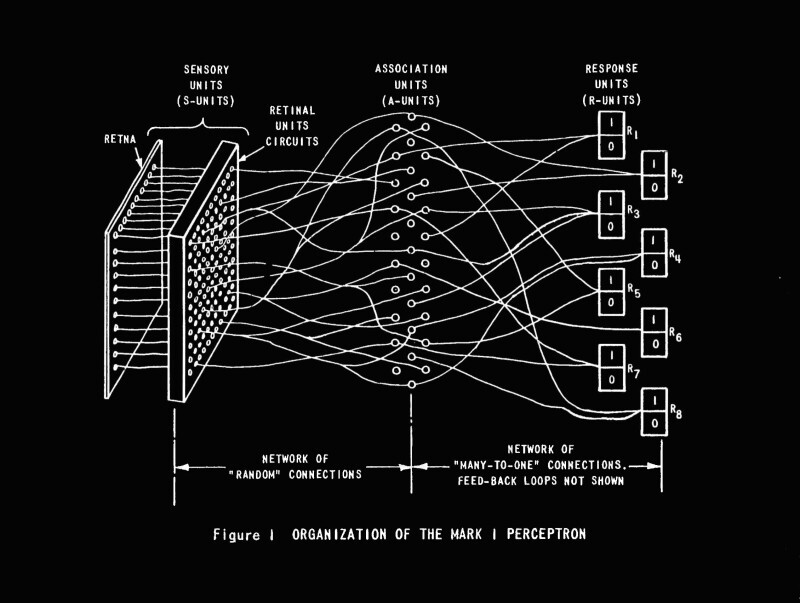
\includegraphics[width=0.45\linewidth]{\toplevelprefix/chapters/chapter1/figs/visu-large.jpg}
    \hspace{2mm} 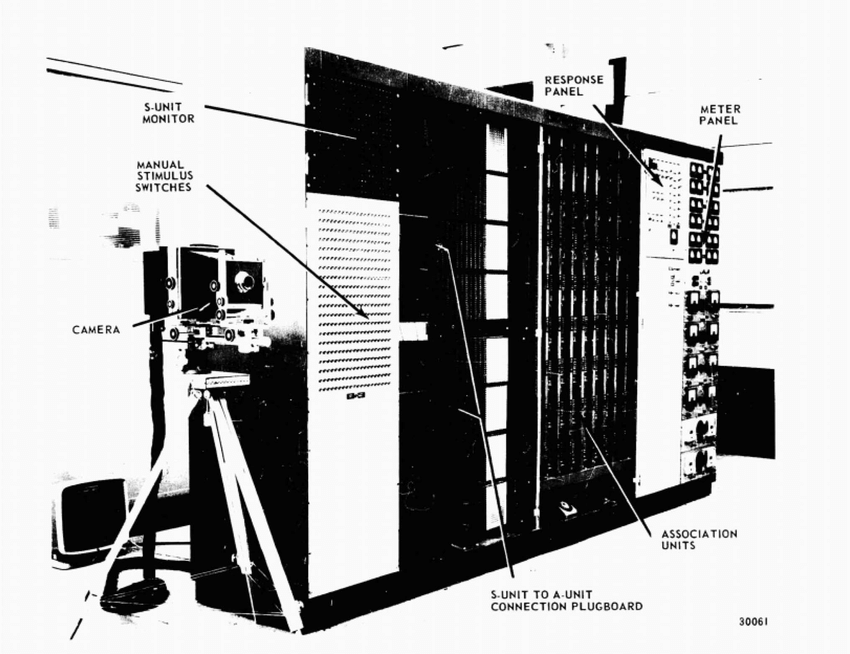
\includegraphics[width=0.45\linewidth]{\toplevelprefix/chapters/chapter1/figs/Original-Mark-I-perceptron-as-seen-in-its-operators-manual-20.ppm.png}
    \caption{The Mark I Perceptron machine developed by Frank Rosenblatt in the late 1950s.}
    \label{fig:perceptron}
\end{figure}


\paragraph{Convolutional neural networks.}
Early experiments with artificial neural networks such as the Mark I Perceptron in the 1950s and 1960s were somewhat disappointing. They suggested that simply connecting neurons in a general fashion, as in multi-layer perceptrons (MLPs), might not suffice. To build effective and efficient networks, it is extremely helpful to understand the collective purpose or function neurons in the network must achieve so that they can be organized and learned in a specialized way. Thus, at this juncture, once again the study of machine intelligence turned to the animal nervous system for inspiration.

It is known that most of our brain is dedicated to processing visual information \cite{PalmerS1999}. In the 1950s and 1960s, David Hubel and Torsten Wiesel systematically studied the visual cortices of cats. They discovered that the visual cortex contains different types of cells---simple cells and complex cells---which are sensitive to visual stimuli of different orientations and locations \cite{Hubel-Wiesel-1959}. Hubel and Wiesel won the 1981 Nobel Prize in Physiology or Medicine for this groundbreaking discovery.

On the artificial neural network side, Hubel and Wiesel's work inspired Kunihiko Fukushima to design the ``neocognitron'' network in 1980, which consists of artificial neurons that emulate biological neurons in the visual cortices \cite{Fukushima1980NeocognitronAS}. This is known as the first \textit{convolutional neural network} (CNN), and its architecture is illustrated in \Cref{fig:neocognitron}. Unlike the perceptron, the neocognitron had more than one hidden layer and could be viewed as a deep network, as shown in \Cref{fig:single-deep} (right).

Also inspired by how neurons work in the cat's visual cortex, Fukushima was the first to introduce the \textit{rectified linear unit} (ReLU):
\begin{equation}
    \varphi(x) = \max\{0, x\} = \casework{x, & \text{if } x > 0, \\ 0, & \text{if } x \leq 0,}
\end{equation}
as the activation function \(\varphi(\cdot)\) in 1969 \cite{Fukushima-1969}. However, it was not until recent years that ReLU became widely used in modern deep (convolutional) neural networks. This book will explain why ReLU is a good choice once we discuss the main operations deep networks implement: compression.

\begin{figure}
    \centering
    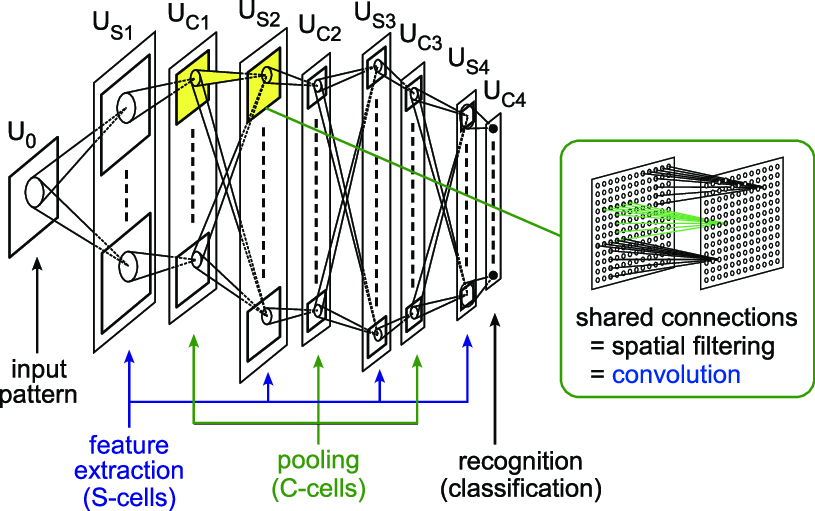
\includegraphics[width=0.6\linewidth]{\toplevelprefix/chapters/chapter1/figs/neocognitron.png}
    \caption{Origin of convolutional neural networks: the Neocognitron by Kunihiko Fukushima in 1980. Notice that the interleaving layers of convolutions and pooling emulate the functions of simple cells and complex cells discovered in the visual cortices of cats.}
    \label{fig:neocognitron}
\end{figure}

CNN-type networks continued to evolve in the 1980s, and many different variants were introduced and studied. However, despite the remarkable capacities of deep networks and the improved architectures inspired by neuroscience, it remained extremely difficult to train such deep networks for real tasks such as image classification. Getting a network to work depended on many unexplainable heuristics and tricks, which limited the appeal and applicability of neural networks. A major breakthrough came around 1989 when Yann LeCun successfully used \textit{back propagation} (BP) to learn a deep convolutional neural network for recognizing handwritten digits \cite{LeCun-1989}, later known as LeNet (see \Cref{fig:LeNet-5}). After several years of persistent development, his perseverance paid off: LeNet's performance eventually became good enough for practical use in the late 1990s \cite{LeCun-1998}. It was used by the US Post Office for recognizing handwritten digits (for zip codes). LeNet was considered the ``prototype'' network for all modern deep neural networks, such as AlexNet \cite{krizhevsky2012imagenet} and ResNet \cite{he2016deep}, which we will discuss later. For this work, Yann LeCun was awarded the 2018 Turing Award.\footnote{Together with two other pioneers of deep networks, Yoshua Bengio and Geoffrey Hinton.}

\begin{figure}
    \centering
    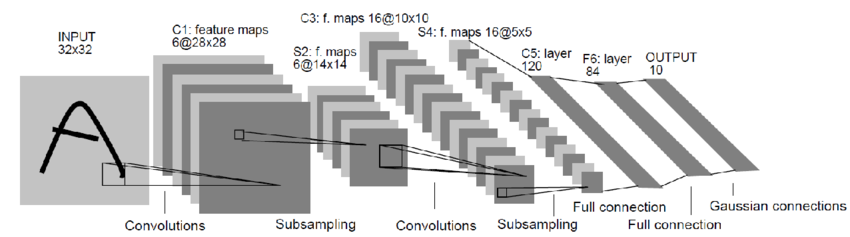
\includegraphics[width=0.95\linewidth]{\toplevelprefix/chapters/chapter1/figs/LeNet-5.png}
    \caption{The LeNet-5 convolutional neural network designed by Yann LeCun in 1989.}
    \label{fig:LeNet-5}
\end{figure}

\paragraph{Backpropagation.}
Throughout history, the fate of deep neural networks has been tied to how easily and efficiently they can be trained. Backpropagation (BP) was introduced for this purpose. A multilayer perceptron can be expressed as a composition of linear mappings and nonlinear activations:
\begin{equation}
    h(\vW_{1}, \ldots, \vW_{L}) = f^{L}(\vW_{L}f^{L-1}(\vW_{L-1} \cdots f^{2}(\vW_{2}f^{1}(\vW_{1}\vx)))).
\end{equation}
To train the network weights \(\{\vW_{l}\}_{l=1}^{L}\) via gradient descent, we must evaluate the gradient \(\partial h/\partial \vW_{l}\). The chain rule in calculus shows that gradients can be computed efficiently for such functions---a technique later termed backpropagation or BP; see \Cref{app:optimization} for details. BP was already known in optimal control and dynamic programming during the 1960s and 1970s, appearing in Paul Werbos's 1974 PhD thesis \cite{Werbos-1974, Werbos1994TheRO}. In 1986, David Rumelhart et al. were the first to apply it to train a multilayer perceptron (MLP) \cite{Rumelhart1986}. Since then, BP has become the dominant technique for training deep networks, as it is scalable and can be efficiently implemented on parallel and distributed computing platforms. However, nature likely does not use BP,\footnote{As we have discussed earlier, nature almost ubiquitously learns to correct errors via closed-loop feedback.} as the mechanism is too expensive for physical implementation.\footnote{End-to-end BP is computationally intractable for neural structures as complex as the brain, especially if the updates need to happen in real time. Instead, localized updates to small sections of the neural circuitry are much more biologically feasible. There is a relatively small amount of work on transplanting such ``local learning'' rules to training deep networks, circumventing BP \cite{baldi2016theory,millidge2022predictive,li2025noprop}. We believe this is an exciting opportunity to improve the scalability of training deep networks.} This leaves ample room for future improvement.

Despite the aforementioned algorithmic advances, training deep networks remained finicky and computationally expensive in the 1980s and 1990s. By the late 1990s, support vector machines (SVMs) \cite{SVM-1995} had gained popularity as a superior alternative for classification tasks.\footnote{Similar ideas for classification problems trace back to Thomas Cover's 1964 PhD dissertation, which was condensed and published in a paper in 1964 \cite{Cover-1964}.} SVMs offered two advantages: a rigorous statistical learning framework known as the Vapnik--Chervonenkis (VC) theory and efficient convex optimization algorithms \cite{BoydVa04}. The rise of SVMs ushered in a second winter for neural networks in the early 2000s.

\paragraph{Compressive auto-encoding.}
In the late 1980s and 1990s, artificial neural networks were already being used to learn low-dimensional representations of high-dimensional data such as images. It had been shown that neural networks could learn PCA directly from data \cite{Oja1982SimplifiedNM,Baldi89}, rather than using the classic methods discussed in \Cref{sec:PCA-ICA}. It was also argued during this period that, due to their ability to model nonlinear transformations, neural networks could learn low-dimensional representations for data with nonlinear distributions. Similar to the linear PCA case, one can simultaneously learn a nonlinear dimension-reduction encoder \(f\) and a decoder \(g\), each modeled by a deep neural network \cite{Rumelhart1986,Kramer1991NonlinearPC}:
\begin{equation}
    \vX   \xrightarrow{\hspace{2mm} f \hspace{2mm}} \vZ  \xrightarrow{\hspace{2mm} g \hspace{2mm}} \hat{\vX}.
       \label{eqn:auto-encoding-deep-networks}
\end{equation}
By enforcing consistency between the decoded data \(\hat{\vX}\) and the original \(\vX\)---for example, by minimizing a MSE-type reconstruction error\footnote{MSE-type errors are known to be problematic for imagery data with complex nonlinear structures. As we will soon discuss, much recent work in generative methods, including GANs, has focused on finding better surrogate distance functions between the original data \(\vX\) and the regenerated \(\hat{\vX}\).}:
\begin{equation}
    \min_{f,g} [\|\vX - \hat{\vX}\|_{2}^{2} = \|\vX - g(f(\vX))\|_{2}^{2}],
\end{equation}
an autoencoder can be learned directly from the data \(\vX\).

But how can we guarantee that such an auto-encoding indeed captures the true low-dimensional structures in \(\vX\) rather than yielding a trivial redundant representation? For instance, one could simply choose \(f\) and \(g\) to be identity maps and set \(\vZ = \vX\). To ensure the auto-encoding is worthwhile, the resulting representation should be compressive according to some computable measure of complexity. In 1993, Geoffrey Hinton and colleagues proposed using coding length as such a measure, transforming the auto-encoding objective into finding a representation that minimizes coding length \cite{Hinton-1993}. This work established a fundamental connection between the principle of minimum description length \cite{Rissanen-1978} and free (Helmholtz) energy minimization. Later work from Hinton's group \cite{Hinton504} empirically demonstrated that such auto-encoding can learn meaningful low-dimensional representations for real-world images. Pierre Baldi provided a comprehensive survey of autoencoders in 2011 \cite{Baldi2011}, just before deep networks gained widespread popularity. We will discuss measures of complexity and auto-encoding further in \Cref{sec:unifying-approach}, and present a systematic study of compressive auto-encoding in \Cref{ch:consistent} from a more unified perspective.

\begin{figure}
    \centering
    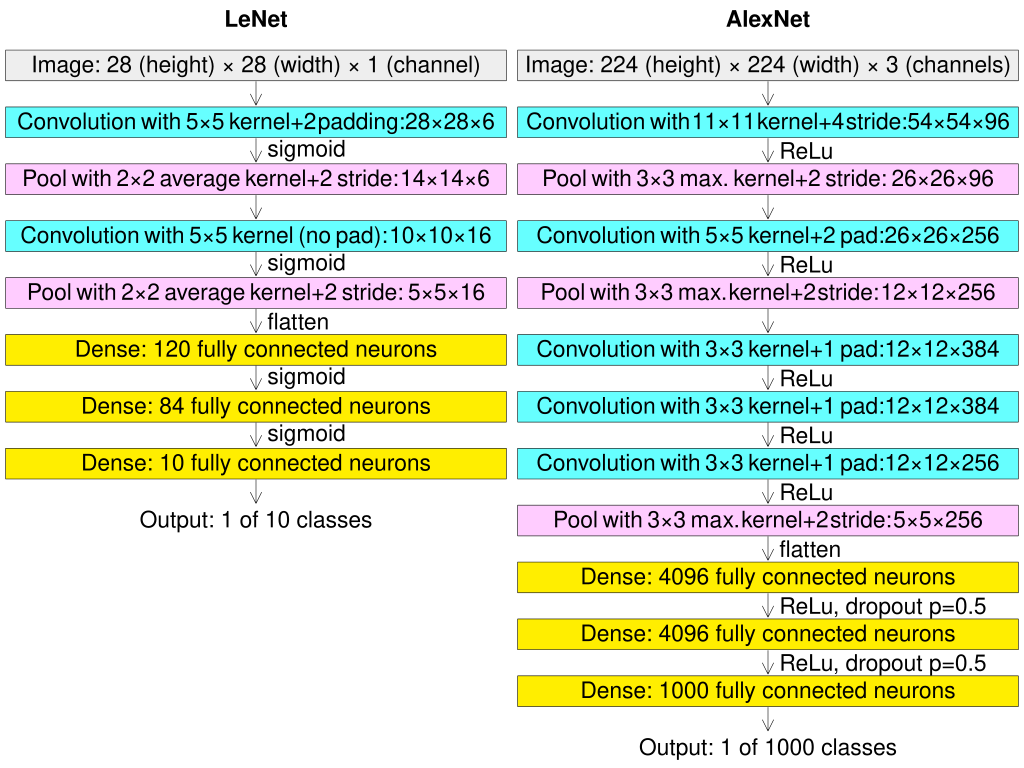
\includegraphics[width=0.8\linewidth]{\toplevelprefix/chapters/chapter1/figs/Comparison_image_neural_networks.svg.png}
    \caption{Architecture of LeNet \cite{LeCun-1989} versus AlexNet \cite{krizhevsky2012imagenet}.}
    \label{fig:LeNet-AlexNet}
\end{figure}


\subsubsection{Modern Deep Neural Networks}
For nearly 30 years---from the 1980s to the 2010s---neural networks were not taken seriously by the mainstream machine learning community. Early deep networks such as LeNet showed promising performance on small-scale classification problems like digit recognition, yet their design was largely empirical, the available datasets were tiny, and back-propagation was computationally prohibitive for the hardware of the era. These factors led to waning interest and stagnant progress, with only a handful of researchers persisting.

\paragraph{Classification and recognition.}
The tremendous potential of deep networks could be unleashed only once sufficient data and computational power became available. By the 2010s, large datasets such as ImageNet had emerged, and GPUs had become powerful enough to make back-propagation affordable even for networks far larger than LeNet. In 2012, the deep convolutional network AlexNet --- named for Alex Krizhevsky, one of the authors \cite{krizhevsky2012imagenet} --- attracted widespread attention by surpassing existing classification methods on ImageNet by a significant margin.\footnote{Deep networks had already achieved state-of-the-art results on speech-recognition tasks, but these successes received far less attention than the breakthrough on image classification.} \Cref{fig:LeNet-AlexNet} compares AlexNet with LeNet. AlexNet retains many characteristics of LeNet---it is simply larger and replaces LeNet's sigmoid activations with ReLUs. This work contributed to Geoffrey Hinton's 2018 Turing Award.

This early success inspired the machine intelligence community to explore new neural network architectures, variations, and improvements. Empirically, it was discovered that larger and deeper networks yield better performance on tasks such as image classification. Notable architectures that emerged include VGG \cite{Simonyan15}, GoogLeNet \cite{Szegedy2014GoingDW}, ResNet \cite{He2016-lc}, and, more recently, Transformers \cite{vaswani2017attention}. Despite rapid empirically-driven performance improvements, theoretical explanations for these architectures---and the relationships among them, if any ---remained scarce. One goal of this book is to uncover the common objective these networks optimize and to explain their shared characteristics, such as multiple layers of linear operators interleaved with nonlinear activations (see \Cref{ch:representation}).

\paragraph{Reinforcement learning.}
Early deep network successes were mainly in supervised classification tasks such as speech and image recognition. Later, deep networks were adopted to learn decision-making or control policies for game playing. In this context, deep networks model the optimal decision/control policy (i.e., a probability distribution over actions to take in order to maximize the expected reward) or the associated optimal value function (an estimate of the expected reward from the given state), as shown in \Cref{fig:Alpha-Go}. Network parameters are incrementally optimized\footnote{Typically via back-propagation (BP).} based on rewards returned from the success or failure of playing the game with the current policy. This learning paradigm is called \textit{reinforcement learning} \cite{Sutton-Barto}; it originated in control-systems practice of the late 1960s \cite{Waltz1965AHA,Mendel1970ReinforcementlearningCA} and traces back through a long and rich history to Richard Bellman's \textit{dynamic programming} \cite{Bellman-DP} and Marvin Minsky's \textit{trial-and-error learning} \cite{Minsky-1954} in the 1950s.

From an implementation standpoint, the marriage of deep networks and reinforcement learning proved powerful: deep networks can approximate control policies and value functions for real-world environments that are difficult to model analytically. This culminated in DeepMind's AlphaGo system, which stunned the world in 2016 by defeating top Go player Lee Sedol and, in 2017, world champion Jie Ke.\footnote{In 1996, IBM's Deep Blue made history by defeating Russian grandmaster Garry Kasparov in chess using traditional machine learning techniques such as tree search and pruning, methods that have proven less scalable and unsuccessful for more complex games like Go.}

AlphaGo's success surprised the computing community, which had long regarded the game's state space as too vast for any efficient solution in terms of computation and sample size. The only plausible explanation is that the optimal value and policy function of Go possess significant favorable structure: qualitatively speaking, their intrinsic dimensions are low enough so that they can be well approximated by neural networks learnable from a manageable number of samples.

\begin{figure}
    \centering
    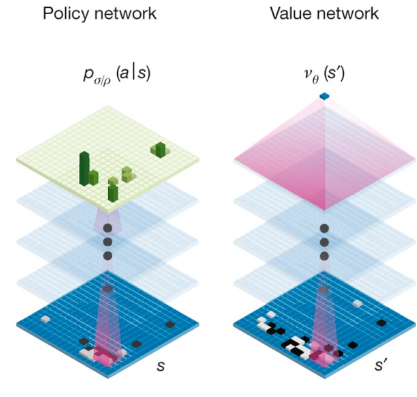
\includegraphics[width=0.5\linewidth]{\toplevelprefix/chapters/chapter1/figs/Policy-Value.png}
    \caption{AlphaGo: using deep neural networks to model the optimal policy or value function for the game Go.}
    \label{fig:Alpha-Go}
\end{figure}

\paragraph{Generation and prediction.}
From a certain perspective, the early practice of deep networks in the 2010s was focused on extracting relevant information from the data \(\vX\) and encoding it into a task-specific representation \(\vZ\) (say \(\vZ\) denotes class labels in classification tasks\footnote{This is a highly atypical notation for labels --- the usual notation is \(\vy\) --- but it is useful for our purposes to consider labels as highly compressed and sparse representations of the data. See \Cref{example:image_classification_feature_learning} for more details.}):
\begin{equation}
    \vX   \xrightarrow{\hspace{2mm} f \hspace{2mm}} \vZ.
       \label{eqn:encoding-deep-networks}
\end{equation}
Here the learned mapping \(f\) needs not preserve most distributional information about \(\vX\); it suffices to retain only the sufficient statistics for the task. For example, a sample \(\vx \in \vX\) might be an image of an apple, mapped by \(f\) to the class label \(\vz = \text{``apple''}\). 

In many modern settings---such as the so-called large general-purpose (``foundation'') models---we may need to also decode \(\vZ\) to recover the corresponding \(\vX\) to a prescribed precision:
\begin{equation}
    \vZ   \xrightarrow{\hspace{2mm} g  \hspace{2mm}} \hat{\vX}.
       \label{eqn:decoding-deep-networks}
\end{equation}
Because \(\vX\) typically represents data observed from the external world, a good decoder allows us to simulate or predict what happens in the world. In a ``text-to-image'' or ``text-to-video'' task, for instance, \(\vz\) is the text describing the desired image \(\vx\), and the decoder should generate an \(\hat{\vx}\) whose content matches \(\vx\). Given an object class \(\vz = \text{``apple''}\), the decoder \(g\) should produce an image \(\hat{\vx}\) that looks like an apple, though not necessarily identical to the original \(\vx\).



\paragraph{Generation via discriminative approaches.}
For the generated images \(\hat{\vX}\) to resemble true natural images \(\vX\), we must be able to evaluate and minimize some distance:
\begin{equation}
    \min \operatorname{dist}(\vX, \hat{\vX}).
\end{equation}
As it turns out, most theoretically motivated distances are extremely difficult---if not impossible---to compute and optimize for distributions in high-dimensional space with low intrinsic dimension.\footnote{This remains true even when a parametric family of distributions for \(\vX\) is specified. The distance often becomes ill-conditioned or ill-defined for distributions with low-dimensional supports. Worse still, the chosen family might poorly approximate the true distribution of interest.}

In 2007, Zhuowen Tu, disappointed by early analytical attempts to model and generate natural images, decided to try a drastically different approach. In a paper published at CVPR 2007 \cite{Tu-2007}, he first suggested learning a generative model for images via a discriminative approach. The idea is simple: if evaluating the distance \(\operatorname{dist}(\vX, \hat{\vX})\) proves difficult, one can instead learn a discriminator \(d\) to separate \(\hat{\vX}\) from \(\vX\):
\begin{equation}
    \begin{tikzpicture}[node distance=1cm, auto]
        \node (Z) {$\Z$};
        \node (Xhat) [right=of Z] {$\hat{\X}$};
        \node (X) [below=of Xhat] {$\X$};
        \node (labels) [right=of Xhat] {$\{0, 1\}$};
        
        \draw[->] (Z) -- (Xhat) node[midway, above] {$g$};
        \draw[->] (Xhat) -- (labels) node[midway, above right] {$d$};
        \draw[->] (X) -- (labels) node[midway, below right] {$d$};
    \end{tikzpicture}
    \label{eqn:gan-networks}
\end{equation}
where labels \(0\) and \(1\) indicate whether an image is generated or real.
Intuitively, the harder it becomes to separate \(\hat{\vX}\) and \(\vX\), the closer they likely are.

Tu's work \cite{Tu-2007} first demonstrated the feasibility of learning a generative model from a discriminative approach. However, the work employed traditional methods for image generation and distribution classification (such as boosting), which proved slow and difficult to implement. After 2012, deep neural networks gained popularity for image classification. In 2014, Ian Goodfellow and colleagues again proposed generating natural images with a discriminative approach \cite{Goodfellow-2014}. They suggested modeling both the generator \(g\) and discriminator \(d\) with deep neural networks. Moreover, they proposed learning \(g\) and \(d\) via a minimax game:
\begin{equation}
    \min_{g} \max_{d} \ell(\vX, \hat{\vX}),
\end{equation}
where \(\ell(\cdot)\) is some natural loss function associated with the classification task. In this formulation, the discriminator \(d\) maximizes its success in separating \(\vX\) and \(\hat{\vX}\), while the generator \(g\) does the opposite. This approach is named \textit{generative adversarial networks} (GANs). It was shown that once trained on a large dataset, GANs can indeed generate photo-realistic images. Partially due to this work's influence, Yoshua Bengio received the 2018 Turing Award.

The discriminative approach appears to cleverly bypass a fundamental difficulty in distribution learning. However, rigorously speaking, this approach does not fully resolve the fundamental difficulty. It is shown in \cite{Goodfellow-2014} that with a properly chosen loss, the minimax formulation becomes mathematically equivalent to minimizing the Jensen-Shannon distance (see \cite{Cover-Thomas}) between \(\vX\) and \(\hat{\vX}\). This remains a hard problem for two low-dimensional distributions in high-dimensional space. Consequently, GANs typically rely on many heuristics and engineering tricks and often suffer from instability issues such as mode collapsing.\footnote{Nevertheless, such a minimax formulation provides a practical approximation of the distance. It simplifies implementation and avoids certain caveats in directly computing the distance.}

\paragraph{Generation via denoising and diffusion.}
In 2015, shortly after GANs were introduced and gained popularity, Surya Ganguli and his students proposed that an iterative denoising process modeled by a deep network could be used to learn a general distribution, such as that of natural images \cite{Sohl-Dickstein2015}. Their method was inspired by properties of special Gaussian and binomial processes studied by William Feller in 1949 \cite{Feller1949OnTT}.\footnote{Again, in the magical era of the 1940s!}

\begin{figure}[t]
    \centering
    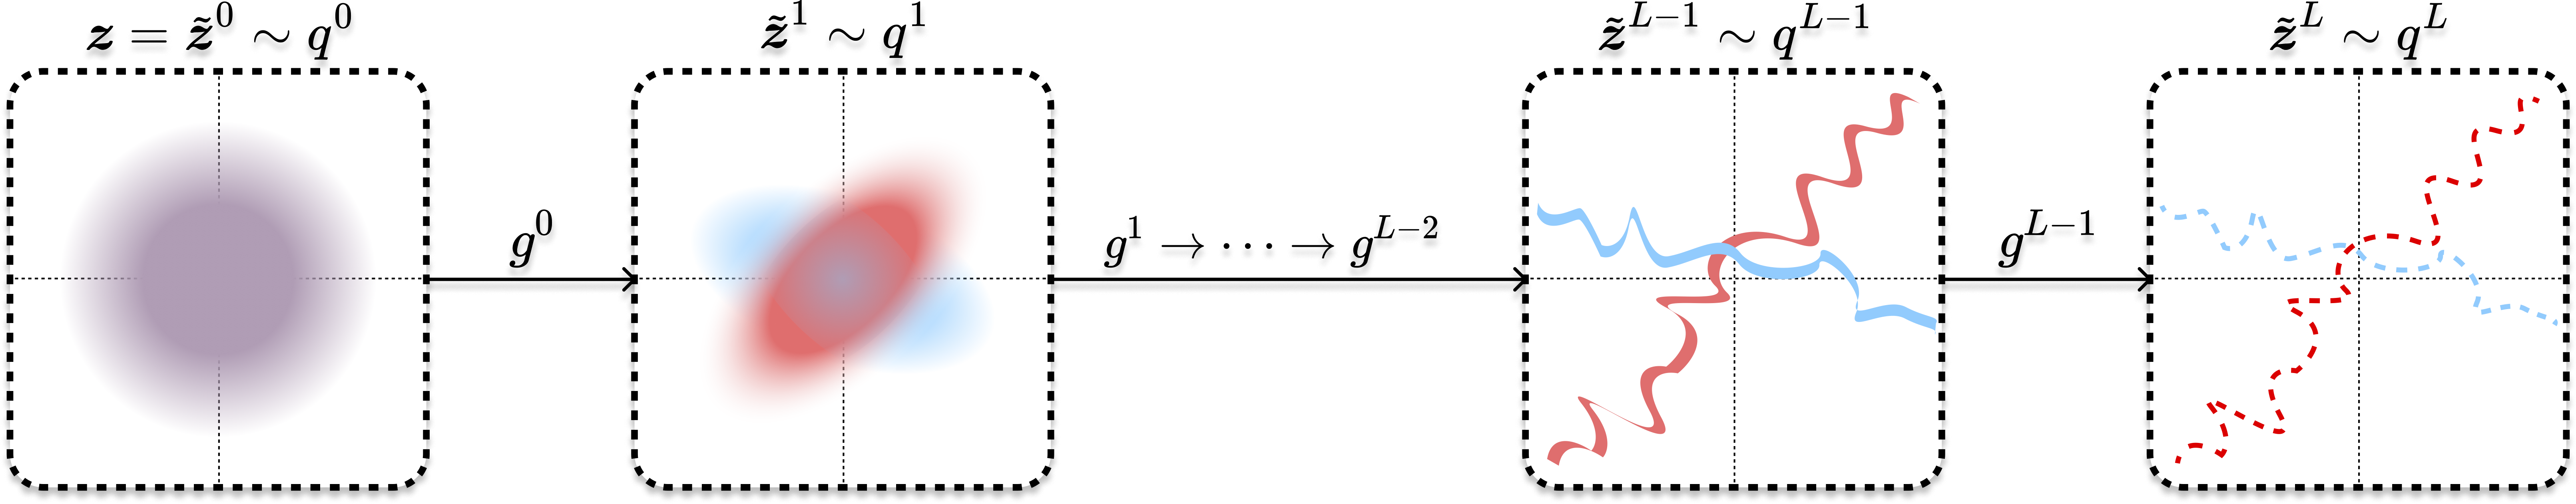
\includegraphics[width=\linewidth]{\toplevelprefix/chapters/chapter1/figs/diffusion_pipeline.png}
    \caption{Illustration of an iterative denoising and compressing process that, starting from a Gaussian distribution \(q^{0} = \mathcal{N}(\vzero, \vI)\), converges to an arbitrary low-dimensional data distribution \(q^{L} = p\).}
    \label{fig:diffusion}
\end{figure}

Soon, denoising operators based on the score function \cite{hyvarinen05a}, briefly introduced in \Cref{sec:denoising-intro}, were shown to be more general and unified the denoising and diffusion processes and algorithms \cite{song2019,song2020score,ho2020denoising}. \Cref{fig:diffusion} illustrates the process that transforms a generic Gaussian distribution \(q^{0} = \mathcal{N}(\vzero, \vI)\) to an (arbitrary) empirical distribution \(p(\vx)\) by performing a sequence of iterative denoising (or compressing) operations:
\begin{equation}
    \vz^{0} \sim  \mathcal{N}(\vzero, \vI) \xrightarrow{\hspace{2mm} g^{0} \hspace{2mm}} \vz^{1} \xrightarrow{\hspace{2mm} g^{1} \hspace{2mm}} \cdots \xrightarrow{\hspace{2mm} g^{L-1} \hspace{2mm}} \vz^{L} \sim p(\vx).
\end{equation}
By now, denoising (and diffusion) has replaced GANs and become the mainstream method for learning distributions of images and videos, leading to popular commercial image generation engines such as Midjourney and Stability.ai. 
In \Cref{ch:compression} we will systematically introduce and study the denoising and diffusion method for learning a general low-dimensional distribution.


\section{A Unifying Approach}\label{sec:unifying-approach}
% Start of Selection
So far, we have given a brief account of the main objective and history of machine intelligence, along with many important ideas and approaches associated with it. In recent years, following the empirical success of deep neural networks, tremendous efforts have been made to develop theoretical frameworks that help us understand empirically designed deep networks---whether specific seemingly necessary components (e.g., dropout \cite{srivastava2014dropout}, normalization \cite{ioffe2015batch,ba2016layer}, attention \cite{vaswani2017attention}) or their overall behaviors (e.g., double descent \cite{belkin2019reconciling}, neural collapse \cite{papyan2020prevalence}).

Motivated in part by this trend, this book pursues several important and challenging goals:
\begin{itemize}
    \item Develop a theoretical framework that yields rigorous mathematical interpretations of deep neural networks.
    \item Ensure correctness of the learned data distribution and consistency with the learned representation.
    \item Demonstrate that the framework leads to performant architectures and guides further practical improvements.
\end{itemize}
In recent years, mounting evidence suggests these goals can indeed be achieved by leveraging the theory and solutions of the classical analytical low-dimensional models discussed earlier (treated more thoroughly in \Cref{ch:classic}) and by integrating fundamental ideas from related fields---namely information/coding theory, control/game theory, and optimization. This book aims to provide a systematic introduction to this new approach.

\subsection{Learning Parsimonious Representations}
\label{sec:computational-approach-compression}
One necessary condition for any learning task to be possible is that the sequences of interest must be \textit{computable}, at least in the sense of Alan Turing \cite{Turing-1936}. That is, a sequence can be computed via a program on a typical computer.\footnote{There are indeed well-defined sequences that are not computable.} In addition to being computable, we require computation to be \textit{tractable}.\footnote{We do not need to consider predicting things whose computational complexity is intractable---say, grows exponentially in the length or dimension of the sequence.} That is, the computational cost (space and time) for learning and computing the sequence should not grow exponentially in length. Furthermore, as we see in nature (and in the modern practice of machine intelligence), for most practical tasks an intelligent system needs to learn what is predictable from massive data in a very high-dimensional space, such as from vision, sound, and touch. Hence, for intelligence we do not need to consider all computable and tractable sequences or structures; we should focus only on predictable sequences and structures that admit \textit{scalable} realizations of their learning and computing algorithms:
\begin{equation}
    \text{\textbf{computable}} \;
   \Longrightarrow \; \text{\textbf{tractable}} \; \Longrightarrow \; 
   \text{\textbf{scalable}}.
\end{equation}

This is because whatever algorithms intelligent beings use to learn useful information must be \textit{scalable}. More specifically, the computational complexity of the algorithms should scale gracefully---typically linear or even sublinear---in the size and dimension of the data. On the technical level, this requires that the operations the algorithms rely on to learn can only utilize oracle information that can be efficiently computed from the data. More specifically, when the dimension is high and the scale is large, the only oracle one can afford to compute is either the first-order geometric information about the data\footnote{such as approximating a nonlinear structure locally with linear subspaces and computing the gradient of an objective function.} or the second-order statistical information\footnote{such as covariance or correlation of the data or their features.}.
The main goal of this book is to develop a theoretical and computational framework within which we can systematically develop efficient and effective solutions or algorithms with such scalable oracles and operations to \textit{learn} low-dimensional structures from the sampled data and subsequently the predictive function.


\paragraph{Pursuing low-dimensionality via compression.}
From the examples of sequences we gave in \Cref{sec:predictability}, it is clear that some sequences are easy to model and compute, while others are more difficult. The computational cost of a sequence depends on the complexity of the predicting function \(f\). The higher the degree of regression \(d\), the more costly it is to compute. The function \(f\) could be a simple linear function, or it could be a nonlinear function that is arbitrarily difficult to specify and compute.

It is reasonable to believe that if a sequence is harder---by whatever measure we choose---to specify and compute, then it will also be more difficult to learn from its sampled segments. Nevertheless, for any given predictable sequence, there are in fact many, often infinitely many, ways to specify it. For example, for the simple sequence \(x_{n+1} = a x_{n}\), we could also define the same sequence with \(x_{n+1} = a x_{n} + b x_{n-1} - b x_{n-1}\).
Hence it would be very useful to develop an objective and rigorous notion of ``complexity'' for any given computable sequence.

Andrey Kolmogorov, a Russian mathematician, was one of the first to define complexity for any computable sequence.\footnote{Many contributed to this notion of sequence complexity, most notably Ray Solomonoff and Greg Chaitin. All three developed algorithmic information theory independently---Solomonoff in 1960, Kolmogorov in 1965 \cite{Kolmogorov1998OnTO}, and Chaitin around 1966 \cite{Chaitin-1966}.} He proposed that among all programs computing the same sequence, the length of the shortest program measures its complexity. This aligns with Occam's Razor---\textit{choose the simplest theory explaining the same observation}. Formally, let \(p\) be a program generating sequence \(S\) on universal computer \(\cU\). The Kolmogorov complexity of \(S\) is:
\begin{equation}
    K(S) = \min_{p\,:\, \cU(p) = S} L(p). 
\end{equation}
Thus, complexity measures how parsimoniously we can specify or compute the sequence. This definition is conceptually important and historically inspired profound studies in computational complexity and theoretical computer science.

The shortest program length represents the ultimate compression of the sequence, quantifying our gain from learning its generative mechanism. However, Kolmogorov complexity is generally uncomputable \cite{Cover-Thomas} and intractable to approximate. Consequently, it has little practical use---it cannot predict learning difficulty or assess how well we have learned.


\paragraph{Computable measure of parsimony.}
For practical purposes, we need an efficiently computable measure of complexity for sequences generated by the same predicting function.\footnote{In practice, we typically care about learning the predicting function \(f\), rather than any particular sequence generated by \(f\).} Note that part of the reason Kolmogorov complexity is not computable is that its definition is non-constructive.

To introduce a computable measure of complexity, we may take a more constructive approach, as advocated by Claude Shannon through the framework of information theory \cite{Shannon-1948,Cover-Thomas}.\footnote{This framework has successfully guided engineering practice in the communication industry for over 80 years.} By assuming the sequence \(S\) is drawn from a probabilistic distribution \(p(S)\), the entropy of the distribution:\footnote{Here we consider differential entropy as we assume the sequence consists of continuous variables. For discrete variables, we would use \(H(S) = - \sum_{i}p(s_{i}) \log p(s_{i})\).}
\begin{equation}
    h(S) \doteq -\int p(s) \log p(s) \odif{s}
    \label{eqn:entropy-definition}
\end{equation}
provides a natural measure of its complexity. This measure also has a natural interpretation as the average number of binary bits needed to encode such a sequence, as we will see in \Cref{ch:compression}.

To illustrate the main ideas of this view, let us take a large number of long sequence segments:
\begin{equation}
    \{S_{1}, S_{2}, \ldots, S_{i}, \ldots, S_{N}\} \subset \R^{D},
\end{equation}
generated by a predicting function \(f\). Without loss of generality, we assume all sequences have the same length \(D\), so each sequence can be viewed as a vector in \(\R^{D}\). We introduce a coding scheme (with a codebook), denoted \(\cE\), that maps every segment \(S_{i}\) to a unique stream of binary bits \(\cE(S_{i})\), and a corresponding decoding scheme \(\cD\) that maps binary bit strings back to sequence segments (say subject to error \(\epsilon \geq 0\) as such an encoding scheme can be lossy). The simplest scheme fills the space spanned by all segments with \(\epsilon\)-balls, as shown in \Cref{fig:coding-schemes}. We then number the balls, and each sequence is encoded as the binary index of its closest ball, while each binary index is decoded back to the center of the corresponding ball. Thus, each segment can be recovered up to precision \(\epsilon\) from its bit stream.
\begin{figure}
    \centering
    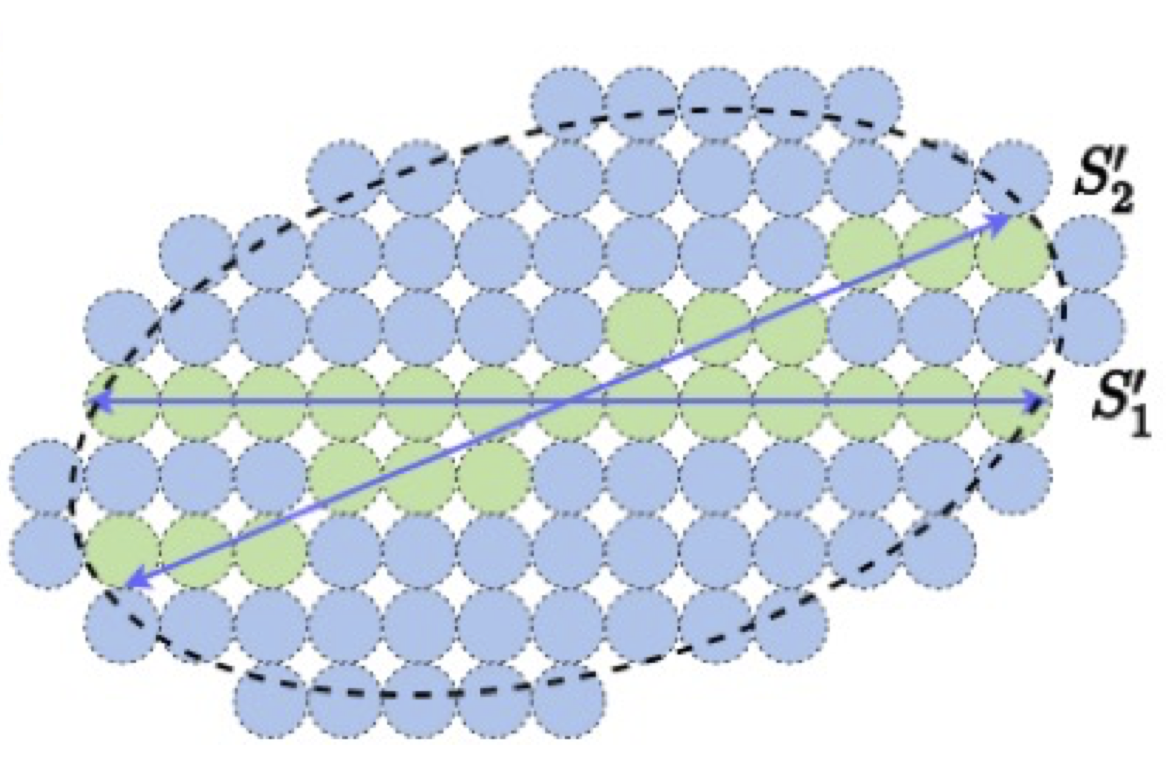
\includegraphics[width=0.5\linewidth]{\toplevelprefix/chapters/chapter1/figs/Coding-schemes.png}
    \caption{Comparison of two coding schemes. Imagine the true data distribution lies along the two arrowed lines. Samples from these lines can be encoded with a codebook of all blue balls, or with a codebook of only the green balls. The second scheme yields a much lower coding length/rate subject to the same precision.}
    \label{fig:coding-schemes}
\end{figure}


Then, for an encoding \(\cE\), the complexity of the predicting function \(f\) can be evaluated as the average coding length \(L(\cE(S))\) of all sequences \(S\) that it generates, known as the coding rate:\footnote{One may make this more precise by taking \(R(S \mid \cE)\) to be the expected coding length for all segments \(S\) of length \(D\).}
\begin{equation}
   R(S \mid \cE) = \Ex[L(\cE(S))] \approx \frac{1}{N}\sum_{i=1}^{N} L(\cE(S_{i})). 
   \label{eqn:coding-rate}
\end{equation}
The coding rate measure will change if we use a different coding scheme (or codebook). In practice, the better we know the low-dimensional structure around which the segments are distributed, the more efficient a codebook we can design, as illustrated in \Cref{fig:coding-schemes}. Astute readers may recognize that conceptually the denoising process illustrated in \Cref{fig:diffusion} closely resembles going from the coding scheme with the blue balls to that with the green ones.

Given two coding schemes \(\cE_{1}\) and \(\cE_{2}\) for the segments, if the difference in the coding rates is positive:
\begin{equation}
   R(S \mid \cE_{1}) -  R(S \mid \cE_{2}) > 0, 
\end{equation}
we may say the coding scheme \(\cE_{2}\) is better. This difference can be viewed as a measure of how much more information \(\cE_{2}\) has over \(\cE_{1}\) about the distribution of the data. To a large extent, the goal of learning the data distribution is equivalent to finding the most efficient encoding and decoding scheme that minimizes the coding rate subject to a desired precision:
\begin{equation}
   \min_{\cE, \cD} R(S \mid \cE) \quad \text{subject to} \quad \operatorname{dist}(S, \cD(\cE(S))) \leq \epsilon. 
\end{equation}
As we will see in \Cref{ch:compression}, the achievable minimal rate is closely related to the notion of entropy \(H(S)\) \eqref{eqn:entropy-definition}.


\begin{remark}\label{rem:computable-complexity}
    The perspective of measuring data complexity with explicit encoding schemes has motivated several learning objectives proposed to revise Kolmogorov complexity for better computability \cite{WallaceC1999}, including the minimum message length (MML) proposed in 1968 \cite{WallaceC1968} and the minimum description length (MDL) in 1978 \cite{Rissanen-1978,HansenM2001}. These objectives normally count the coding length for the coding scheme \(\cE\) itself (including its codebook) in addition to the data \(S\) of interest: \(L(\cE(S)) + L(\cE)\). However, if the goal is to learn a finite-sized codebook and apply it to a large number of sequences, the amortized cost of the codebook can be ignored since
    \begin{equation}
        \frac{1}{N}\left( L(\cE) + \sum_{i=1}^{N} L(\cE(S_{i}))\right) \approx \frac{1}{N}\sum_{i=1}^{N} L(\cE(S_{i}))
    \end{equation}
    as \(N\) becomes large.
\end{remark}

Again, one may view the resulting optimal coding scheme as the one that achieves the best compression of the observed data. In general, compared to the Kolmogorov complexity, the coding length given by any encoding scheme will always be larger:
\begin{equation}
    K(S) < L(\cE(S)).
\end{equation}
Therefore, minimizing the coding rate/length essentially minimizes an upper bound of the otherwise uncomputable Kolmogorov complexity.

\subsection{Learning Informative Representations}
If the goal were simply to compress the given data for its own sake, the optimal codes approaching Kolmogorov complexity would in theory become nearly random or structureless \cite{Chaitin-1966}.\footnote{Any codes with structure can be further compressed.} However, our true purpose in learning the data distribution of sequences $S$ is to use it repeatedly with ease in future predictions. Hence, while compression allows us to identify the low-dimensional distribution in the data, we would like to encode this distribution in a \textit{structured and organized} way so that the resulting representation is informative and efficient to use.\footnote{For example, to sample the distribution under different conditions.} \Cref{fig:expansion} illustrates intuitively why such a transformation is desirable.

\begin{figure}
    \centering
    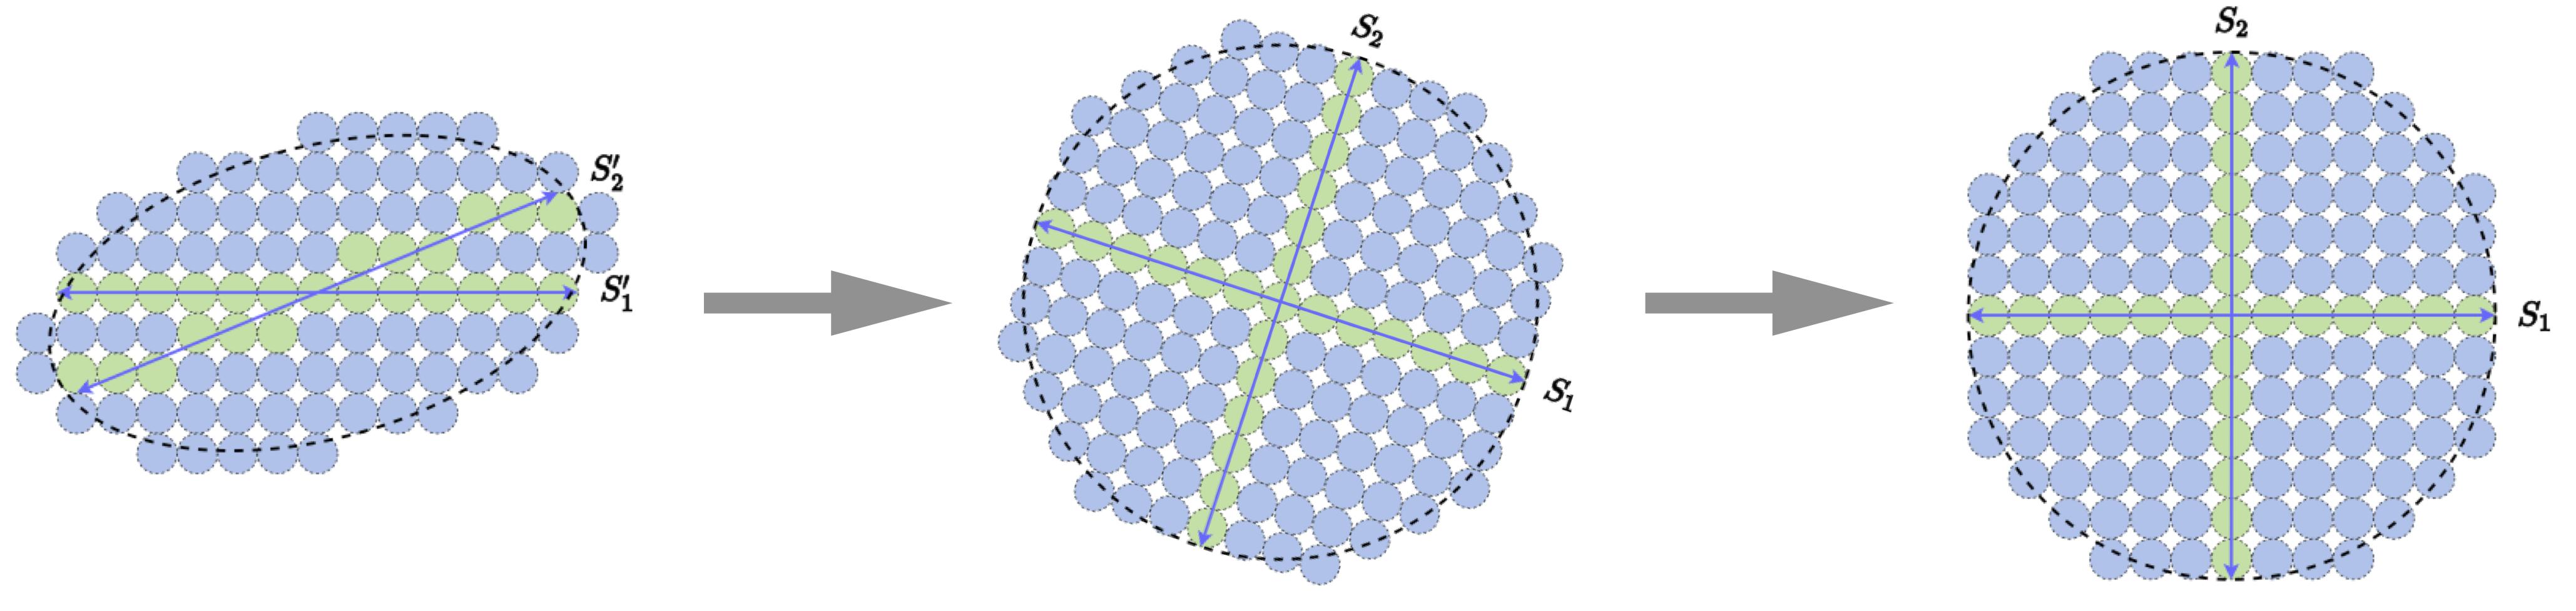
\includegraphics[width=0.98\linewidth]{\toplevelprefix/chapters/chapter1/figs/coding-transform.png}
    \caption{Transforming the identified low-dimensional data distribution into a more informative and structured representation.}
    \label{fig:expansion}
\end{figure}
As we will show in \Cref{ch:compression}, these desired structures in the final representation can be precisely promoted by choosing a natural measure of \textit{information gain} based on the coding rates of the chosen coding schemes.\footnote{The information gain is a pervasive idea in algorithmic information theory and has been incorporated in several approaches to this topic, most recently \(\mathcal{V}\)-information \cite{xu2020theory}. This particular instantiation, similarly to many other measures of complexity we discussed, suffers from being increasingly poorly-conditioned as the data support becomes more compact and low-dimensional, and so is not suitable for our needs.} Throughout this book, such an explicit and constructive coding approach provides a powerful computational framework for learning good representations of low-dimensional structures in real-world data. In many cases of practical importance, the coding length function can be efficiently computed or accurately approximated. In some benign cases, we can even obtain closed-form formulae---for example, subspace and Gaussian models (see \Cref{ch:compression}).

Moreover, this computational framework leads to a principled approach that naturally reveals the role deep networks play in this learning process. As we will derive systematically in \Cref{ch:representation}, the layers of a deep network perform operations that incrementally optimize the objective function of interest. From this perspective, the role of deep networks can be precisely interpreted as emulating a certain iterative optimization algorithm---say, gradient descent---to optimize the objective of information gain. Layers of the resulting deep architectures can be endowed with precise statistical and geometric interpretations, namely performing incremental compressive encoding and decoding operations. Consequently, the derived deep networks become transparent ``white boxes'' that are mathematically fully explainable.



\subsection{Learning Consistent Representations}

\label{sec:consistency}

To summarize our discussions so far, let us denote the data as
\begin{equation}
    \vX = \{S_{1}, S_{2}, \ldots, S_{i}, \ldots, S_{N}\} \subset \R^{D},
\end{equation}
and let \(\vZ = \cE(\vX)\) be the codes of \(\vX\) via some encoder \(\cE\):
\begin{equation}
    \vX  \xrightarrow{\hspace{2mm} \cE\hspace{2mm}} \vZ.
    \label{eqn:open-loop}
\end{equation}
In the machine learning context, \(\vZ\) is often called the ``features'' of \(\vX\). Note that without knowing the underlying distribution of \(\vX\), we do not know which encoder \(\cE\) should be used to retain the most useful information about the distribution of \(\vX\). In practice, people often start by trying a compact encoding scheme that serves a specific task well. In particular, they try to learn an encoder that optimizes a certain (empirical) measure of parsimony for the learned representation:
\begin{equation}
    \min \rho(\vZ). 
\end{equation}

\begin{example}\label{example:image_classification_feature_learning}
    For example, image classification is such a case: we assign all images in the same class to a single code and images in different classes to different codes, say ``one-hot'' vectors:
    \begin{equation}
        \vx \mapsto \vz \in \{  [1, 0, 0, \ldots , 0, 0], \;  [0, 1, 0 \ldots, 0, 0], \; \ldots, \;  [0,0,0, \ldots, 0, 1].\}
        \label{eqn:class-labels}
    \end{equation}
    Now, a classifier \(f(\cdot)\) can be modeled as a function that predicts the probability of a given \(\vx\) belonging to each of the \(k\) classes: \(\hat{\vz} = f(\vx) \in \R^{K}\). Then the ``goodness'' of a classifier can be measured by the so-called {\em cross entropy}:\footnote{The cross entropy can be viewed as a distance measure between the ground truth distribution of \(\vz\) and that of the prediction \(\hat{\vz}\). It can also be viewed as the expected coding length of \(\vz\) if we use the optimal code book for \(\hat{\vz}\) to encode \(\vz\). The cross entropy reaches its minimum when \(\vz\) and \(\hat{\vz}\) have the same distribution.}
    \begin{equation}
        \ell(\hat{\vz}, \vz) = \sum_{k=1}^{K} - z_{k} \log \hat{z}_{k},
    \end{equation}
    where \(z_{k}\) indicates the \(k\)-th entry of the vector \(\vz\). As the early practice of deep networks indicated \cite{krizhevsky2012imagenet}, if enough data are given, such an encoding scheme can often be represented by a deep network and learned in an end-to-end fashion by optimizing the cross-entropy. 
\end{example}

The cross-entropy loss \(\ell(\hat{\vz}, \vz)\) can be viewed as a special measure of parsimony \(\rho(\vz)\) associated with a particular family of encoding schemes that are suitable for classification. However, such an encoding is obviously \textit{very lossy}. The learned \(\vz\) does not contain any other information about \(\vx\) except for its class type. For example, by assigning an image with (a code representing) the class label ``apple'', we no longer know which specific type of apple is in the original image from the label alone. 

Of course, the other extreme is to require the coding scheme to be \textit{lossless}. That is, there is a one-to-one mapping between \(\vx\) and its code \(\vz\). However, as we will see in \Cref{ch:compression}, lossless coding (or compression) is impractical unless \(\vx\) is discrete. For a continuous random variable, we may only consider lossy coding schemes so that the coding length for the data can be finite. That is, we only encode the data up to a certain prescribed precision. As we will elaborate more in \Cref{ch:compression}, lossy coding is not merely a practical choice; it plays a fundamental role in making learning of the underlying continuous distribution possible from finite samples of the distribution. 

For many learning purposes, we want the feature \(\vz\), although \textit{lossy}, to retain more information about \(\vx\) than just its class type. In this book, we will introduce a more general measure of parsimony based on coding length/rate associated with a more general family of coding schemes---coding with a mixture of subspaces or Gaussians. This family has the capability to closely approximate arbitrary real-world distributions up to a certain precision. As we will see in \Cref{ch:compression} and \Cref{ch:representation}, such a measure will not only preserve most information about the distribution of \(\vX\) but will also promote certain desirable geometric and statistical structures for the learned representation \(\vZ\). 


\paragraph{Bidirectional auto-encoding for consistency.}
In a broader learning context, the main goal of a compressive coding scheme \(\cE\) is to identify the low-dimensional structures in the data \(\vX\) so that they can be used to predict things in the original data space. This requires that the learned encoding scheme \(\cE\) admits an efficient decoding scheme, denoted \(\cD\), which maps the feature or encoded data \(\vZ\) back to the data space:
\begin{equation}
    \vX   \xrightarrow{\hspace{2mm} \cE\hspace{2mm}} \vZ  \xrightarrow{\hspace{2mm} \cD \hspace{2mm}} \hat{\vX}.
       \label{eqn:auto-encoding}
\end{equation}
We call such an encoding--decoding pair \((\cE, \cD)\) an \textit{auto-encoding}. \Cref{fig:autoencoder} illustrates this process.
\begin{figure}
    \centering
    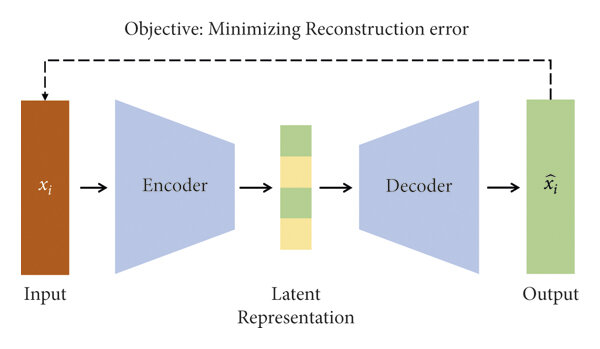
\includegraphics[width=0.7\linewidth]{\toplevelprefix/chapters/chapter1/figs/Autoencoder.jpg}
    \caption{Illustration of the architecture of an autoencoder.}
    \label{fig:autoencoder}
\end{figure}

Ideally, the decoding is approximately an ``inverse'' of the encoding, so that the data (distribution) \(\hat{\vX}\) decoded from \(\vZ\) is similar to the original data (distribution) \(\vX\) to some extent.\footnote{We will make precise what we mean by ``similar'' later.} If this holds, we can recover or predict from \(\vZ\) what occurs in the original data space. In this case, we say the pair \((\cE, \cD)\) provides a \textit{consistent} auto-encoding. For most practical purposes, we not only need such a decoding to exist, but also need it to be efficiently realizable and physically implementable. For example, if \(\vx\) is real-valued, quantization is required for any decoding scheme to be realizable on a finite-state machine, as we will explain in \Cref{ch:compression}. Thus, in general, realizable encoding and decoding schemes are necessarily lossy. A central question is how to learn a compact (lossy) representation \(\vZ\) that can still predict \(\vX\) well.

Generally speaking, both the encoder and decoder can be modeled and realized by deep networks and learned by solving an optimization problem of the following form:
\begin{equation}
   \min_{f, g} [\ell(\vX, \hat{\vX}) + \rho(\vZ)], \qquad \text{where} \quad \vZ = f(\vX), \quad \hat{\vX} = g(\vZ)
   \label{eqn:auto-encoding-objective}
\end{equation}
where \(\ell(\cdot, \cdot)\) is a distance function that promotes similarity between \(\vX\) and \(\hat{\vX}\)\footnote{Either sample-wise or distribution-wise, depending on the choice of \(\ell\).} and \(\rho(\vZ)\) is a measure that promotes parsimony and information richness of \(\vZ\). The classic principal component analysis (PCA) \cite{JolliffeI2002} is a typical example of a consistent auto-encoding, which we will study in great detail in \Cref{ch:classic}, as a precursor to more general low-dimensional structures. In \Cref{ch:auto-encoding}, we will study how to learn consistent auto-encoding for general (say nonlinear) low-dimensional distributions.  


\subsection{Learning Self-Consistent Representations}
In the auto-encoding objective above, one must evaluate how close the decoded data \(\hat{\vX}\) is to the original \(\vX\). This typically requires external supervision or knowledge of an appropriate similarity measure. Computing similarity between \(\hat{\vX}\) and \(\vX\) can be prohibitively expensive, or even impossible.\footnote{For instance, minimizing a distributional distance between the two random variables is statistically and computationally difficult.} In nature, animals learn autonomously without comparing their estimate \(\hat{\vX}\) with the ground truth \(\vX\) in the data space; they typically lack that option.\footnote{In animals and humans, the eyes process visual data long before it arrives at the brain; the brain does not have a mechanism to process raw visual data and must rely on the eyes' features to do any learning.}

How, then, can a system learn without external supervision or comparison? How can it know that \(\hat{\vX}\) is consistent with \(\vX\) without direct comparison? This leads to the idea of ``closing the loop.'' Under mild conditions (made precise in \Cref{ch:closed-loop}), ensuring consistency between \(\vX\) and \(\hat{\vX}\) reduces to encoding \(\hat{\vX}\) as \(\hat{\vZ}\) and checking consistency between \(\vZ\) and \(\hat{\vZ}\). We call this notion \textit{self-consistency}, illustrated by:
\begin{equation}
    \vX   \xrightarrow{\hspace{2mm} \cE\hspace{2mm}} \vZ  \xrightarrow{\hspace{2mm} \cD \hspace{2mm}} \hat{\vX} \xrightarrow{\hspace{2mm} \cE\hspace{2mm}} \hat{\vZ},
    \label{eqn:closed-loop}
\end{equation}
We call this process \textit{closed-loop transcription},\footnote{Inspired by transcription between DNA and RNA or other proteins.} depicted in \Cref{fig:closed-loop}.

\begin{figure}[t]
    \centering
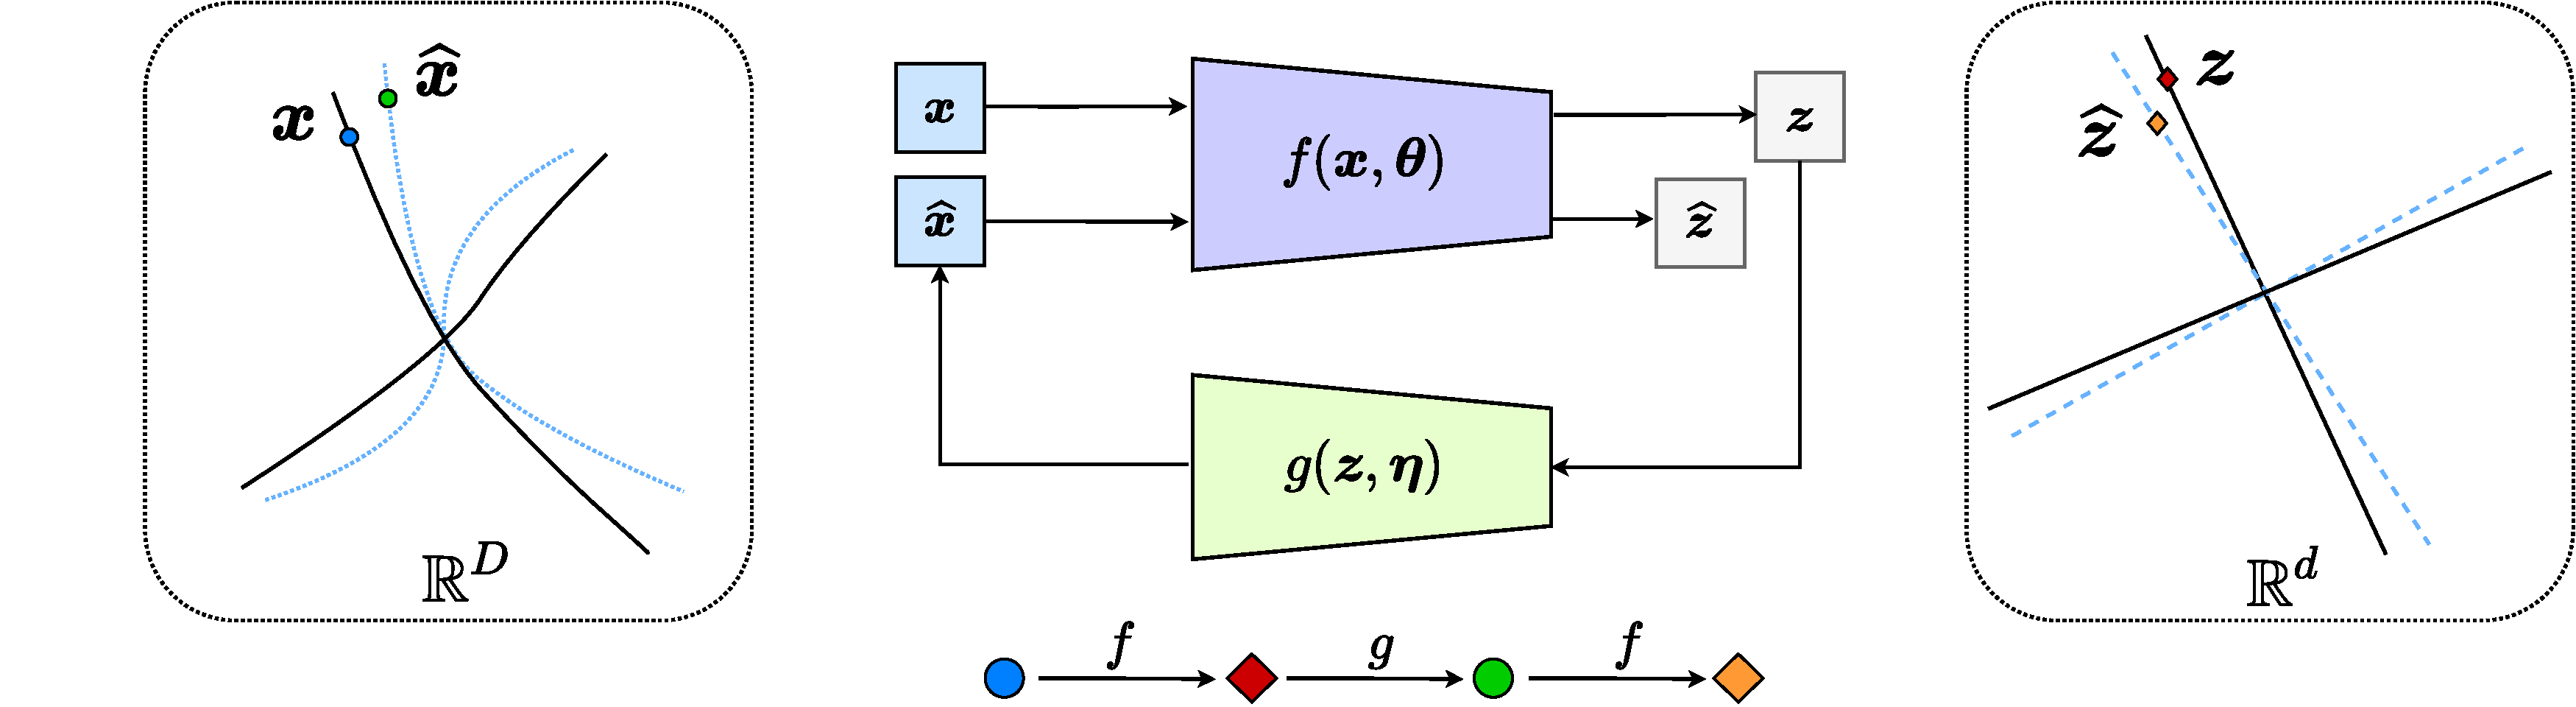
\includegraphics[width=0.9\linewidth]{\toplevelprefix/chapters/chapter1/figs/diagrams_redu_gan_2.pdf}
\caption{Illustration of a closed-loop transcription. Here we use a mapping \(f\) to represent the encoder \(\cE\) and \(g\) to represent the decoder \(\cD\).}  \label{fig:closed-loop}
\end{figure}

It is arguably true that any autonomous intelligent being only needs to learn a self-consistent representation \(\vZ\) of the observed data \(\vX\), because checking consistency in the original data space---often meaning in the external world---is either too expensive or even physically infeasible. The closed-loop formulation allows one to learn an optimal encoding \(f(\cdot, \vtheta)\) and decoding \(g(\cdot, \veta)\) via a min-max game that depends only on the internal (learned) feature \(\vZ\):
\begin{equation}
    \max_{\vtheta}\min_{\veta} [\ell( \vZ, \hat{\vZ}) + \rho(\vZ)],  \qquad \text{where} \quad \vZ = f(\vX), \quad \hat{\vX} = g(\vZ), \quad \hat{\vZ} = f(\hat{\vX}) 
   \label{eqn:closed-loop-objective}
\end{equation}
where \(\ell( \vZ, \hat{\vZ})\) is a loss function based on coding rates of the features \(\vZ\) and \(\hat{\vZ}\), which, as we will see, can be much easier to compute. Here again, \(\rho(\vZ)\) is some measure that promotes parsimony and information richness of \(\vZ\). Somewhat surprisingly, as we will see in \Cref{ch:closed-loop}, under rather mild conditions such as \(\vX\) being sufficiently low-dimensional, self-consistency between \((\vZ, \hat{\vZ})\) implies consistency in \((\vX, \hat{\vX})\)! In addition, we will also see that a closed-loop system will allow us to learn the distribution in a \textit{continuous and incremental} manner,\footnote{That is, to learn with one class at a time or even one sample at a time.} without suffering from problems such as catastrophic forgetting associated with open-loop models.

% Start of Selection
\section{Bridging Theory and Practice for Machine Intelligence}
So far, we have introduced three related frameworks for learning a compact and structured representation \(\vZ\) for a given data distribution \(\vX\):
\begin{itemize}
    \item the open-ended encoding \eqref{eqn:open-loop};
    \item the bi-directional auto-encoding \eqref{eqn:auto-encoding};
    \item the closed-loop transcription \eqref{eqn:closed-loop}.
\end{itemize}
In this book, we will systematically study all three frameworks, one after another:
\begin{equation}
    \text{\textbf{open-ended}} \; \Longrightarrow \; 
    \text{\textbf{bi-directional}} \; \Longrightarrow \; \text{\textbf{closed-loop}},
\end{equation}
in \Cref{ch:representation}, \Cref{sec:consistent-representation} and \Cref{sec:self-consistency} of \Cref{ch:auto-encoding}, respectively

In recent years, many theoretical frameworks have been proposed to help understand deep networks. However, most have failed to provide scalable solutions that match the performance of empirical methods on real-world data and tasks. Many theories offer little practical guidance for further empirical improvement. \Cref{ch:conditional-inference} and \Cref{ch:applications} will demonstrate how the framework presented in this book can bridge the gap between theory and practice. \Cref{ch:conditional-inference} will show how to use the learned distribution and its representation to conduct (Bayesian) inference for practical tasks involving (conditional) generation, estimation, and prediction. \Cref{ch:applications} will provide compelling experimental evidence that networks and systems designed from first principles can achieve competitive---and potentially superior---performance on tasks such as visual representation learning, image classification, image completion, segmentation, and text generation.

\paragraph{Back to intelligence.}
As mentioned at the beginning, a fundamental task of any intelligent being is to learn predictable information from sensed data. We now understand the computational nature of this task and recognize that it is never-ending for two reasons:
\begin{itemize}
    \item Knowledge learned from data, say via encoding and decoding schemes, is unlikely to be correct or optimal. Intelligence must be able to improve when predictions of new observations contain errors.
    \item Observed data do not yet cover all predictable information. Intelligence must recognize when current knowledge is inadequate and acquire new information whenever it becomes available.
\end{itemize}

Thus, intelligence is \textit{not} about collecting all data in advance and training a model to memorize predictable information. Instead, it requires computational mechanisms that continuously improve current knowledge and acquire new information when needed. A fundamental characteristic of any intelligent being or system---whether an animal, human, robot, scientific community, or civilization---is \textit{the ability to continuously improve or gain information on its own}. We can symbolically express the relationship between intelligence and information as:
\begin{equation}
    \operatorname{Intelligence}(t) = \odv*{\operatorname{Information}}{t}(t), \qquad 
    \operatorname{Information}(t)  = \int_{0}^{t} \operatorname{Intelligence}(s) \odif{s}.
\end{equation}
The closed-loop framework provides a universal mechanism for self-improvement and self-learning through feedback---reinforcement being a primitive form, as in natural selection---or gaming, with scientific inquiry representing its most advanced form through hypothesis formulation and verification. All intelligent beings and systems in nature employ closed-loop mechanisms for learning at every level and scale. This ubiquity inspired early attempts to model intelligence with machines and computers, particularly the Cybernetics movement initiated by Norbert Wiener in the 1940s.

We hope this book helps readers better understand the objectives, principles, and computational mechanisms underlying intelligence. It lays the groundwork for future study of higher-level human intelligence---true artificial intelligence. We will outline several significant open problems in these directions in \Cref{ch:future}.

\end{document}
